% !TeX program = xelatex
\documentclass[12pt,a4paper]{article}
\usepackage[margin=1in]{geometry}
\usepackage{iftex}
\ifPDFTeX
  \usepackage[T1]{fontenc}
  \usepackage[utf8]{inputenc}
  \usepackage{newtxtext}
\else
  \usepackage{fontspec}
  \setmainfont{Times New Roman}
\fi
\usepackage[british]{babel}
\usepackage{amsmath,amssymb}
\usepackage{graphicx}
\usepackage{booktabs,tabularx,longtable,array}
\usepackage{microtype}
\usepackage{setspace}
\usepackage{titlesec}
\usepackage{caption}
\usepackage{csquotes}
\usepackage[backend=biber,style=apa,sortcites=true]{biblatex}
\DeclareLanguageMapping{british}{british-apa}
\addbibresource{Paper2C_hr_attrition_references.bib}
\usepackage[hidelinks]{hyperref}
\usepackage{xurl}
\hypersetup{pdfauthor={},pdftitle={The epistemic fragility of people analytics: How evaluation leakage, construct invalidity, and algorithmic isomorphism distort strategic retention decisions}}

\newif\ifanonymous
\anonymoustrue
\newcommand{\ManuscriptWordCount}{8350}
\setlength{\parindent}{0.5in}
\setlength{\parskip}{0pt}
\setlength{\emergencystretch}{1em}
\setlength{\LTpre}{\baselineskip}
\setlength{\LTpost}{\baselineskip}
\renewcommand{\arraystretch}{1.2}
\setlength{\bibhang}{0.5in}
\setlength{\bibitemsep}{0pt}
\titleformat{\section}{\normalfont\normalsize\bfseries}{}{0pt}{}
\titleformat{\subsection}{\normalfont\normalsize\bfseries\itshape}{}{0pt}{}
\captionsetup{font=small,labelfont=bf,justification=raggedright,singlelinecheck=false}
\renewenvironment{abstract}{\section*{Abstract}\noindent\ignorespaces}{\par}
\title{The epistemic fragility of people analytics: How evaluation leakage, construct invalidity, and algorithmic isomorphism distort strategic retention decisions}
\author{}
\date{}

\begin{document}
\doublespacing
\begin{titlepage}
\centering
\vspace*{1cm}
{\bfseries The epistemic fragility of people analytics: How evaluation leakage, construct invalidity, and algorithmic isomorphism distort strategic retention decisions\par}
\vspace{1cm}
Anonymous manuscript\par
Human Resource Management Journal\par
\vspace{1cm}
Approximate word count: \ManuscriptWordCount\par
\small Main text, tables and captions; excluding abstract, references and appendix.\par
\normalsize
\vfill
Author details are provided separately for editorial use.\par
\end{titlepage}

\begin{abstract}
Drawing on institutional legitimacy theory, algorithmic management, and voluntary turnover research, this study problematises the epistemic foundation of predictive attrition analytics. As human resource (HR) functions face mimetic and normative pressures to demonstrate analytical sophistication, a small set of public datasets has become the de facto evidence base for claims that employee departures are predictable with near-certainty. Across a systematic methodological audit of 20 published attrition studies and a controlled factorial evaluation of six public workforce tables, seven classifier families, and four over-sampling methods, we demonstrate that this evidence base is compromised by two compounding failures: evaluation leakage and construct invalidity. Applying synthetic over-sampling before partitioning development and hold-out data inflates reported minority-class F1 by 0.235 (95\% CI 0.226--0.244), from 0.591 to 0.826, and doubles reported performance on the ubiquitous IBM HR benchmark (from 0.434 to 0.877)---an artefact nearly twice as large as the spread across algorithm families (0.129). Crucially, a psychometric and structural audit reveals why honest discrimination remains bounded and why appending employee-attitude and attendance records on a widely used corporate case study fails to improve valid prediction: the 4,410-row table is an IBM-sized replica (exactly three times IBM's row and leaver counts, with identical univariate distributions) in which 1,442 of 1,498 unique complete profiles are repeated three times, so a random split leaks duplicate records (correct F1 falls from 0.708 to 0.322 after deduplication), and single-item ordinal labels lack the longitudinal shock and embeddedness processes that govern turnover. We theorise how deploying uncalibrated, leakage-inflated algorithms distorts retention resource allocation and triggers self-fulfilling psychological contract breaches through false-positive surveillance, and we advance HR-SAFE as a strategic algorithmic governance framework to rebalance institutional authority between HR leaders, line managers, and technical vendors.
\end{abstract}
\noindent\textbf{Keywords:} HR analytics; algorithmic HRM; institutional legitimacy; voluntary employee turnover; construct validity; strategic algorithmic governance

\clearpage
\section{Introduction}
People analytics has been widely promoted as a catalyst for evidence-based human resource management (HRM), yet critical scholarship increasingly questions whether its rapid proliferation reflects genuine decision value or an institutional quest for scientific legitimacy \parencite{ref50,ref44,ref51,ref56}. A decade after \textcite{ref50} warned that HR was set to fail the `big data' challenge by ceding domain authority to technical specialists, foundational reviews continue to document a persistent chasm between computational elaboration and verified organisational impact \parencite{ref44,ref57,ref52}. As predictive algorithms move from experimental dashboards into high-stakes employment decisions---governing who is monitored, counselled, or offered scarce retention resources---the epistemic quality of algorithmic evidence becomes a core strategic HRM responsibility rather than a peripheral information-technology concern \parencite{ref45,ref54,ref58,ref53}.

Nowhere is this tension more acute than in predictive employee-attrition modelling. Framed as a clean binary classification task, turnover prediction has attracted an expansive applied literature and commercial vendor ecosystem claiming that individual departures can be forecast with minority-class F1 scores and accuracies approaching 0.95 to 0.99 \parencite{ref1,ref2,ref3,ref23,ref24}. Because longitudinal, multi-wave enterprise HR information system (HRIS) records are rarely shared publicly due to confidentiality and data-protection constraints \parencite{ref52,ref64}, a small set of open-access tables---most notably the IBM Watson HR Analytics benchmark---has come to function as the field's de facto evidence base. Published research, executive business cases, and vendor demonstrations routinely invoke these benchmark scores to assert that employee turnover is a largely solved prediction problem. If that corpus is structurally flawed, however, the peril is not merely that a specific statistical model is overfitted; it is that strategic HRM is anchoring its retention architecture and professional legitimacy on a quantified illusion \parencite{ref51,ref60}.

Drawing on institutional isomorphism \parencite{ref59,ref51}, algorithmic control theory \parencite{ref58,ref61}, and century-long voluntary turnover scholarship \parencite{ref36,ref46,ref48,ref62}, we argue that the prevailing attrition-analytics corpus suffers from two distinct but mutually reinforcing threats: \textit{evaluation contamination} and \textit{construct invalidity}. First, because departing employees constitute a minority class in annual workforce snapshots, analysts routinely apply synthetic over-sampling techniques such as the Synthetic Minority Over-sampling Technique (SMOTE) \parencite{ref5,ref6,ref7} to rebalance the data. When synthetic interpolation is executed across the entire dataset prior to partitioning development and evaluation samples, artificial profiles that are near-copies of future hold-out employees are injected directly into the training partition. The resulting test no longer measures generalisation to unseen employees; it rewards memorisation of contaminated neighbours \parencite{ref12,ref13,ref14,ref21}.

Second, and more fundamentally for HRM scholarship, a public spreadsheet labelled `attrition' is not thereby a valid psychometric or longitudinal representation of voluntary, regrettable organisational exit \parencite{ref36,ref62}. Close inspection of the public corpus reveals severe construct pathology: the dominant IBM HR benchmark is an undocumented synthetic demonstration table; a widely reused technology dataset actually captures external labour-market job search rather than internal organisational turnover; two regional datasets are near-balanced cross-sectional extracts; and a prominent 4,410-row corporate `case study' shipping with employee-survey, manager-survey, and daily attendance logs is, as we demonstrate below, an IBM-sized replica: it has exactly three times IBM's $n$ and leaver counts and the same univariate distributions, and 1,442 of its 1,498 unique complete-attribute profiles are exact triplicate rows, but the records are not row-wise copies of IBM HR. When construct invalidity is compounded by evaluation leakage, high headline metrics mask the theoretical reality that static HRIS records cannot capture the dynamic relational shocks, unfolding decision paths \parencite{ref46}, psychological contract breaches \parencite{ref47}, and job embeddedness sacrifices \parencite{ref48} that drive actual departures.

To establish the magnitude and managerial consequences of these twin failures, we combine a systematic methodological audit of 20 peer-reviewed attrition studies with a controlled experimental factorial across six public workforce tables, seven classifier families, four over-sampling methods, ten random seeds, and three evaluation protocols that vary solely in where resampling sits relative to the train--test partition. We further conduct targeted construct-validity and psychometric audits---isolating external labour-market mobility, joining multi-source attitude and attendance records, and deduplicating cloned employee profiles---alongside hyperparameter tuning, probability calibration, and cost-sensitive retention accounting.

This study makes three primary contributions to the HR analytics and strategic HRM literature. First, we theorise and empirically quantify the \textit{quantified illusion} in people analytics, demonstrating that pre-partition resampling inflates minority-class F1 by an average of 0.235 (and doubles the IBM HR score from 0.434 to 0.877), an evaluation artefact nearly twice as large as the 0.129 performance spread across seven machine-learning algorithm families. Second, we bridge voluntary turnover theory and machine-learning methodology by exposing the psychometric and structural limits of public HR benchmarks: we show that appending single-item survey and attendance columns fails to improve honest discrimination, and that stripping duplicate complete-attribute profiles in the case-study table (from 4,410 rows to 1,498 unique profiles) collapses its correctly evaluated F1 from 0.708 to 0.322. Third, we move beyond technical critique to examine how uncalibrated, false-positive-laden risk scores threaten employee well-being, personal integrity, and psychological contracts through algorithmic surveillance \parencite{ref61,ref60}, and we advance HR-SAFE as a strategic algorithmic governance framework that empowers HR leaders to reclaim evaluative authority over predictive retention systems.

\section{Theoretical framework and literature review}
\subsection{Institutional legitimacy, algorithmic isomorphism, and the epistemic crisis in HR analytics}
\label{sec:people-analytics}
Evidence-based management rests on the premise that managerial decisions should be informed by the conscientious, explicit, and judicious use of the best available scientific evidence \parencite{ref43}. Within HRM, however, the institutionalisation of people analytics has been shaped as much by sociopolitical pressures for professional legitimacy as by verified improvements in workforce decision-making \parencite{ref50,ref44,ref51}. Historically marginalized in strategic boardroom deliberations, HR functions face intense institutional pressures---coercive, mimetic, and normative \parencite{ref59}---to adopt the quantitative vocabulary and algorithmic tools of finance and operations \parencite{ref50,ref56}. \textcite{ref51} conceptualise HR analytics adoption as a multi-stage legitimacy process wherein pragmatic, moral, and cognitive legitimacy are pursued through the deployment of seemingly objective dashboards and predictive scores. Crucially, cognitive legitimacy can be achieved when an analytical practice becomes taken for granted as `state-of-the-art science', even when the underlying empirical evidence is fragile or unverified \parencite{ref44,ref52}.

We term this phenomenon \textit{algorithmic isomorphism}: the mimetic convergence of academic researchers, commercial HR-technology vendors, and internal analytics teams around standardised machine-learning pipelines and benchmark datasets that project an aura of predictive omniscience. As \textcite{ref54} argue, artificial intelligence in HR is characterised by deep paradoxes: the same algorithmic systems marketed to enhance objectivity and strategic agility can simultaneously degrade work quality, marginalise human judgement, and entrench opaque vendor narratives. When HR professionals lack the methodological literacy to interrogate how predictive scores are produced \parencite{ref50,ref56}, an epistemic asymmetry emerges. Technical specialists and external vendors control the modelling pipeline, while HR leaders consume headline accuracy or F1 figures at face value to justify retention budgets and algorithmic interventions \parencite{ref45,ref55,ref53}.

In algorithmic HRM, this epistemic gap carries direct consequences for organisational control and employee relations. \textcite{ref58} demonstrate that workplace algorithms operate as a contested terrain of control through mechanisms of recording, rating, and recommending. When an attrition model assigns departure probabilities to identifiable employees, it does not merely describe the workforce; it enacts a rating regime that alters how managers perceive and treat subordinates \parencite{ref61,ref60}. Because human capital outcomes are socially constructed, causally complex, and relatively rare \parencite{ref45}, a predictive claim in HRM requires rigorous validation of both its statistical generalisability and its underlying measurement constructs \parencite{ref56,ref53}. Examining the production process of published attrition scores is therefore central to establishing credible human capital analytics.

\subsection{Voluntary turnover theory and the construct limits of static HRIS prediction}
\label{sec:turnover-theory}
A century of organisational psychology and HRM scholarship establishes that voluntary employee turnover is a dynamic, context-dependent relational process unfolding over time, rather than a deterministic function of static demographic and payroll attributes \parencite{ref36,ref62}. In their foundational unfolding model, \textcite{ref46} demonstrated that employees rarely leave through a single linear calculation of job dissatisfaction; instead, departures follow distinct psychological paths frequently triggered by `shocks'---jarring external or internal events such as an unsolicited job offer, a merger, a passed-over promotion, or a family relocation---that prompt image violations and script-driven exits. Complementing this process view, psychological contract theory highlights that withdrawal is heavily governed by employees' subjective beliefs regarding reciprocal obligations and perceived breaches of trust by the employer \parencite{ref47}. Conversely, job embeddedness theory explains why employees remain: individuals are tethered to their organisations and communities through a web of formal and informal links, perceived person--environment fit, and the material or psychological sacrifices that departure would entail \parencite{ref48}.

Synthesising this theoretical canon reveals a fundamental epistemological boundary for predictive people analytics. Meta-analytic evidence across decades of turnover research shows that even well-validated, multi-item psychometric measures of job attitudes, organisational commitment, and embeddedness yield moderate effect sizes, leaving substantial variance in individual departure behaviour unexplained \parencite{ref36,ref62}. Routine cross-sectional HRIS extracts---recording age, tenure, salary band, commute distance, and occasional single-item ratings---capture neither exogenous labour-market shocks \parencite{ref46} nor the relational fabric of embeddedness and psychological contract fulfilment \parencite{ref47,ref48}. Furthermore, operational HR decisions require distinguishing between voluntary and involuntary exits, and between dysfunctional (regrettable) loss of high performers and functional turnover \parencite{ref20,ref36}.

Turnover theory therefore provides a powerful theoretical lens for evaluating machine-learning claims in HRM. Because employee exit is governed by unobserved temporal shocks, subjective contract evaluations, and multi-layered embeddedness, static cross-sectional HR tables possess an inherent information ceiling. When published studies or commercial vendors report near-perfect individual classification (e.g., F1 $> 0.90$) on cross-sectional HR data, turnover theory implies that such figures should be treated not as breakthroughs in behavioural prediction, but as prima facie symptoms of methodological contamination or construct artifice \parencite{ref36,ref45,ref64}.

\subsection{Class imbalance, probability calibration, and the pre-partition leakage mechanism}
\label{sec:imbalance}
The technical catalyst for evaluation contamination in attrition modelling lies in how analysts handle class imbalance. In most organisations, annual voluntary turnover ranges between 5\% and 20\% of the workforce. Standard classification algorithms optimising overall accuracy on skewed data tend to favour the majority class (stayers), achieving high nominal accuracy while failing to identify departing employees. To counter this, the applied attrition literature has overwhelmingly adopted synthetic resampling---predominantly SMOTE \parencite{ref5,ref27} and its adaptive or borderline extensions \parencite{ref6,ref7}---as a mandatory preprocessing step \parencite{ref23,ref24,ref29,ref26}.

Yet methodological research across biostatistics and machine learning has increasingly challenged the uncritical use of class-imbalance corrections. \textcite{ref8} demonstrated that SMOTE is largely ineffective in high-dimensional feature spaces, while \textcite{ref11} showed that for strong, properly tuned classifiers, synthetic balancing rarely improves discrimination beyond what is achievable by adjusting the decision threshold. More critically for managerial decision-making, \textcite{ref9} and \textcite{ref10} proved that artificial rebalancing systematically destroys probability calibration: by forcing the training prevalence toward 50\%, models trained on SMOTE-balanced data produce severely overestimated risk probabilities. In strategic HRM, probability calibration is vital \parencite{ref41,ref42,ref25}: if a retention dashboard reports that an employee has an 80\% probability of quitting when the true empirical incidence among comparable staff is 20\%, any cost--benefit calculation governing retention bonuses or career interventions will systematically misallocate organisational resources \parencite{ref20,ref34}.

\begin{center}
[Figure~\ref{fig:1} near here]
\end{center}

Compounding the calibration penalty is a pervasive protocol error concerning \textit{when} resampling is executed. SMOTE generates synthetic minority records by selecting an observed leaver and interpolating feature values along the line segment connecting that employee to their $k$-nearest minority neighbours \parencite{ref5}. As illustrated in Figure~\ref{fig:1}, if this interpolation is performed on the complete dataset \textit{before} partitioning into training and hold-out test sets, two forms of data leakage occur simultaneously \parencite{ref12,ref13,ref14,ref21}. First, synthetic employees created as weighted averages of a specific leaver end up in the training partition while the real employee is assigned to the hold-out test set; the classifier need only recognise a near-duplicate rather than generalise to an independent cohort. Second, the test partition itself becomes populated with synthetic interpolations, altering the evaluation distribution from a realistic workforce prevalence (e.g., 16\% leavers) to an artificial 50:50 balance. While recent technical notes on the IBM HR dataset have advocated confining SMOTE to cross-validation folds and observed much lower F1 scores of 0.439 to 0.504 \parencite{ref15,ref16}, the HRM literature lacks a systematic audit of how deeply this protocol error and construct invalidity have distorted the field's evidence base.

\section{Data and method}
\subsection{Forensic construct audit of the public attrition corpus}
To evaluate the evidence base on which published attrition analytics rests, we examine six widely used public workforce tables (Table~\ref{tab:1}), encompassing 14,876 nominal records across diverse organisational and national contexts. Rather than treating these files as interchangeable representations of organisational turnover, we first conduct a forensic construct and psychometric audit of their origin, measurement structure, and record independence. Each dataset is then harmonised using a standardised, leakage-free preprocessing pipeline: administrative identifiers and zero-variance constants (`EmployeeCount`, `StandardHours`, `Over18`, `EmployeeNumber`) are removed, categorical attributes are one-hot encoded, missing numeric values are median-imputed, and the minority class (leavers) is coded as positive. No pre-split feature selection is performed, ensuring that variable screening does not introduce a secondary channel of information leakage \parencite{ref12,ref13}.

\begin{center}
[Table~\ref{tab:1} near here]
\end{center}

Our forensic audit exposes four critical construct limitations across the public corpus that have been largely overlooked in prior reviews \parencite{ref23,ref24}:
\begin{enumerate}
\item \textbf{Synthetic demonstration schemas (\texttt{ibm\_hr} and \texttt{healthcare\_attr}):} The flagship IBM HR dataset ($n = 1470$, 237 leavers, imbalance ratio [IR] = 5.20) is not an empirical HRIS extract from a real enterprise; it is an artificial dataset created by IBM Watson data scientists to demonstrate software capabilities. Its attitudinal variables (`JobSatisfaction`, `EnvironmentSatisfaction`, `RelationshipSatisfaction`, `WorkLifeBalance`, `JobInvolvement`) are single-item ordinal integers ($1\text{--}4$) lacking multi-item psychometric reliability, temporal ordering, or differentiation between voluntary and involuntary exits. In these data, point-biserial correlations between attitudinal items and attrition are uniformly weak ($r = -0.046$ to $-0.130$), and `PerformanceRating` exhibits virtually zero association with departure ($r = 0.003$). The healthcare table ($n = 1676$, IR = 7.42) is an IBM-style public variant of the same schema family.
\item \textbf{Duplicate-profile leakage and multi-file artifice (\texttt{hr\_case\_study}):} A heavily cited Kaggle corporate case study ($n = 4410$, 711 leavers, IR = 5.20) distributes a core demographic table (\texttt{general\_data}) alongside separate employee-survey, manager-survey, and daily office badge in/out timestamp logs. Each of the 4,410 rows has a distinct \texttt{EmployeeID}, so this is not a repeated-ID panel. Deduplicating on every non-identifier attribute, however, yields 1,498 unique complete profiles: 1,442 appear three times, 28 twice, and 28 once. Row count and leaver count are exactly three times IBM HR ($3 \times 1470 = 4410$; $3 \times 237 = 711$), and univariate counts of age, department, gender, job role, and attrition match IBM exactly, with monthly income recorded on a ten-fold scale; row-wise overlap with IBM HR is nevertheless zero, including after dividing income by ten. Employee-survey ratings are not identical within all triplicate groups (18--34 groups disagree on satisfaction or work--life items); manager ratings are. Under a standard random train--test split of the 4,410 rows, copies of the same complete-attribute profile can sit on both sides of the split, creating duplicate-record leakage even before SMOTE is applied. We retain the raw 4,410-row table in the baseline six-table comparison to reflect how published studies use it, and we then isolate both the multi-file survey/attendance join and the 1,498-profile deduplicated table in dedicated construct checks.
\item \textbf{External labour-market mobility (\texttt{job\_change\_ds}):} Recording data scientists registered with a training provider ($n = 5000$ stratified subsample from 19,158 records, IR = 3.01), this table captures whether candidates are seeking a new employer in the external labour market rather than internal organisational attrition. Because published HR studies routinely pool it as an attrition benchmark \parencite{ref18}, we evaluate the corpus both with and without it.
\item \textbf{Near-balanced cross-sectional extracts (\texttt{turnover\_russia} and \texttt{saudi\_attrition}):} The Russian dataset ($n = 1129$, IR = 1.02) and the primary survey of Saudi private-sector employees ($n = 1191$, IR = 1.31; \cite{ref4}) provide genuine empirical observations, including perceptual survey items in the Saudi sample, but their near-50:50 class balance diverges sharply from typical annual organisational turnover rates.
\end{enumerate}

\subsection{Experimental design: Three protocols, one structural difference}
To isolate the pure causal effect of evaluation protocol on reported model performance, every comparison in our primary factorial holds the dataset, feature encoding, classification algorithm, hyperparameters, over-sampling technique, 70:30 stratified partition ratio, and random number seeds strictly constant. Only the position of the synthetic over-sampler varies across three conditions:
\begin{itemize}
\item \textbf{Leaked protocol (pre-split resampling):} The over-sampler is fitted and applied to the complete dataset first, and the resulting rebalanced data are then partitioned 70:30 into training and test sets.
\item \textbf{Correct protocol (post-split, train-only resampling):} The original dataset is partitioned 70:30 first; the over-sampler is embedded inside an `imbalanced-learn` pipeline \parencite{ref22} and applied strictly to the 70\% training partition, leaving the 30\% test partition composed entirely of untouched real records at their natural workforce prevalence.
\item \textbf{No-resampling baseline:} The original dataset is partitioned 70:30 and the classifier is fitted on the natural training distribution without synthetic rebalancing.
\end{itemize}

Because every other modelling choice is identical, any divergence between the leaked and correct scores is attributable to the protocol ordering. We cross these three protocols across seven canonical classifier families---logistic regression (LogReg), decision tree (DecTree), 5-nearest neighbours (5NN), radial-basis-function support vector machine (SVM-RBF), random forest (RandForest), gradient boosting (GradBoost), and extreme gradient boosting (XGBoost)---and four over-sampling methods: SMOTE \parencite{ref5}, Borderline-SMOTE \parencite{ref6}, ADASYN \parencite{ref7}, and Random Over-Sampling (RandomOS), replicated across 10 random seeds.\footnote{The six HR tables are drawn from a broader methodological programme examining resampling protocols across general classification benchmarks; all analyses, construct audits, psychometric joins, calibration tests, and governance frameworks presented here are developed specifically for the HRM domain.} Complete technical specifications, hyperparameter grids, random seeds, and software package versions are documented in Appendix~\ref{app:technical}.

\subsection{Evaluation metrics, construct robustness checks, and systematic literature audit}
We evaluate models across complementary metrics tailored to HR decision-making. Minority-class F1 (the harmonic mean of precision and recall for leavers) is our primary outcome because it dominates published attrition benchmarks. Because F1 ignores true negatives (correctly identified stayers), we also compute the Matthews correlation coefficient (MCC), which incorporates all four cells of the confusion matrix \parencite{ref17}, and average precision (AP, area under the precision--recall curve), which summarises ranking quality across all possible decision thresholds \parencite{ref30,ref37}.

To address potential methodological and HRM objections, we execute four additional empirical investigations:
\begin{enumerate}
\item \textbf{Psychometric join and profile deduplication on \texttt{hr\_case\_study}:} We merge the ignored employee-survey (`EnvironmentSatisfaction`, `JobSatisfaction`, `WorkLifeBalance`), manager-survey (`JobInvolvement`, `PerformanceRating`), and daily badge attendance files (fraction of missing in/out timestamps and recorded days) onto \texttt{general\_data}, expanding the feature space from 33 to 42 encoded columns. We evaluate LogReg, RandForest, and XGBoost with SMOTE across 10 seeds under all three protocols on both the standard 4,410-row table and the table deduplicated to 1,498 unique complete-attribute profiles.
\item \textbf{Hyperparameter tuning under leaked versus correct validation:} To test whether the protocol gap is merely an artefact of library-default hyperparameters, we run a 12-iteration randomised search (`RandomizedSearchCV`, 3-fold inner cross-validation, 5 seeds) on RandForest and XGBoost for IBM HR, comparing honest inner-fold SMOTE against pre-resampled tuning, and scoring the leaked-tuned models on both synthetic and real hold-out labels.
\item \textbf{Probability calibration and cost-sensitive retention accounting:} Across 10 stratified 70:30 hold-outs on IBM HR, we evaluate predicted departure probabilities against observed frequencies using Brier scores \parencite{ref32} and reliability diagrams \parencite{ref31,ref41}, and we translate confusion-matrix counts into an illustrative utility-analysis cost account \parencite{ref20,ref35} assuming a 10:1 replacement-to-intervention cost ratio.
\item \textbf{Systematic methodological audit of published attrition studies:} Expanding beyond anecdotal comparisons, we audit 20 peer-reviewed employee-attrition studies (2018--2026) across five evidentiary dimensions aligned with our governance framework: dataset construct (synthetic IBM vs.\ real HRIS), resampling method, stated partition ordering (`before-split`, `train-only`, or `not stated`), baseline reporting, and probability calibration assessment.
\end{enumerate}

\section{Results}
\subsection{The quantified illusion: Protocol contamination versus algorithmic choice}
Across the six public workforce tables, applying synthetic over-sampling prior to the train--test split inflates reported minority-class F1 by an average of 0.235 (bootstrap 95\% CI 0.226--0.244), elevating mean performance from an honest 0.591 under the correct protocol to 0.826 under the leaked protocol (Table~\ref{tab:2}). To place this magnitude in managerial perspective, the performance spread between the strongest and weakest of the seven machine-learning algorithm families---correctly evaluated and averaged across datasets, samplers, and seeds---is 0.129 (ranging from 0.512 for 5-nearest neighbours to 0.641 for random forest; XGBoost is also 0.641). Changing the evaluation protocol thus alters the headline evidence presented to HR decision-makers nearly twice as much as changing the underlying prediction algorithm.

\begin{center}
[Table~\ref{tab:2} near here]
\end{center}

\begin{center}
[Figure~\ref{fig:2} near here]
\end{center}

As Table~\ref{tab:2} and Figure~\ref{fig:2} demonstrate, this inflation is not distributed uniformly across datasets; it concentrates precisely where workforce imbalance resembles realistic annual turnover. On the near-balanced Russian (\texttt{turnover\_russia}, IR = 1.02) and Saudi (\texttt{saudi\_attrition}, IR = 1.31) extracts, the leakage premium is negligible (0.0026 and 0.0460, respectively). As the proportion of leavers falls toward realistic organisational rates, the leaked score detaches sharply from honest generalisation, reaching a premium of 0.3672 on \texttt{healthcare\_attr} (IR = 7.42) and 0.4425 on the flagship \texttt{ibm\_hr} benchmark (IR = 5.20). Across the six tables, the leakage premium correlates with the log imbalance ratio at $r = 0.9195$. On IBM HR, pre-partition resampling multiplies the honest F1 score (0.4342) by a factor of 2.02 (to 0.8767).

\begin{center}
[Figure~\ref{fig:3} near here]
\end{center}

The mathematical mechanism driving this divergence is direct. When leavers represent only 12\% to 16\% of the workforce, an over-sampler must manufacture three to six synthetic minority records for every real leaver to achieve class parity. When this synthesis occurs prior to partitioning, the feature space around every real leaver is densely populated with interpolated clones that cross the train--test boundary. Across the broader benchmark reference distribution (Figure~\ref{fig:3}), honest F1 declines as class imbalance deepens, whereas leaked F1 rises artificially because the test set becomes progressively dominated by synthetic interpolations.

Table~\ref{tab:3} confirms that this distortion is not an idiosyncrasy of the F1 metric. When evaluated using Matthews correlation (Panel A) and threshold-free average precision (Panel B) on the exact same model fits, pre-split resampling inflates MCC by 0.210 on average (and by 0.409 on IBM HR, from 0.346 to 0.755) and inflates AP by 0.257 (and by 0.470 on IBM HR, from 0.461 to 0.931). Under the correct protocol, mean MCC across the six workforce tables is 0.444 (ranging from 0.262 to 0.571), indicating moderate rank-ordering capability suitable for cohort-level triage rather than individual-level certainty.

\begin{center}
[Table~\ref{tab:3} near here]
\end{center}

Crucially, comparing the `No resampling' and `Correct' columns of Table~\ref{tab:2} resolves a practical modelling question frequently bypassed in people analytics: whether to resample at all. Unlike high-dimensional biomedical benchmarks where resampling often fails \parencite{ref8}, correctly confined train-only resampling improves mean F1 over the unresampled baseline on all six HR tables, yielding an average gain of 0.064 F1 points (winning 79.8\% of matched comparisons, with the unresampled baseline winning 20.2\%). However, because this gain reflects a shift in the precision--recall trade-off at the default 0.5 threshold rather than creation of new behavioural information, reporting the unresampled baseline alongside any resampled model remains essential due diligence.

\subsection{Deconstructing construct validity: Labour-market mobility, psychometric survey joins, and cloned employee profiles}
\label{sec:construct-results}
A critical HRM reviewer might ask whether the 0.235 protocol premium is an artefact of pooling heterogeneous constructs, or whether incorporating richer attitudinal and behavioural HR measures would eliminate the gap and restore high predictive accuracy. Table~\ref{tab:7} reports our multi-stage construct and psychometric audit, which reveals that isolating employer-style schemas and auditing record structure sharpens rather than diminishes our findings.

\begin{center}
[Table~\ref{tab:7} near here]
\end{center}

First, removing the external labour-market mobility table (\texttt{job\_change\_ds}, which shows a premium of 0.256 on its own) leaves an internal-turnover premium of 0.231 (95\% CI 0.221--0.241) across the five employer-style datasets. Restricting further to the three IBM-like schemas (\texttt{ibm\_hr}, \texttt{healthcare\_attr}, and \texttt{hr\_case\_study})---the exact data structure that dominates published HR analytics---raises the protocol inflation to 0.350 (95\% CI 0.342--0.359), lifting mean F1 from 0.548 (correct) to 0.898 (leaked).

Second, we examine the corporate case study (\texttt{hr\_case\_study}) by joining its unused employee-survey (`EnvironmentSatisfaction`, `JobSatisfaction`, `WorkLifeBalance`), manager-survey (`JobInvolvement`, `PerformanceRating`), and daily badge attendance summaries onto \texttt{general\_data} (expanding encoded features from 33 to 42). Evaluated across LogReg, RandForest, and XGBoost with SMOTE on the published 4,410-row table, adding these nine HR-specific attitude and attendance columns leaves honest F1 completely unchanged at 0.708 (33 features) versus 0.707 (42 features; MCC = 0.648 vs.\ 0.651), while the leaked protocol reports 0.892 and 0.900 (premiums of 0.184 [95\% CI 0.145--0.223] and 0.193 [95\% CI 0.160--0.226]).

Why does the 4,410-row case study achieve a seemingly respectable `correct' F1 of 0.708 when IBM HR, which has the same class balance and matching univariate counts, scores only 0.434, and why do survey and attendance variables add zero predictive lift? The bottom two rows of Table~\ref{tab:7} provide the forensic answer. Deduplicating \texttt{hr\_case\_study} on every non-identifier column yields 1,498 unique complete-attribute profiles (1,442 of them appearing three times). A standard 70:30 random split of the raw 4,410 rows can therefore place copies of the same profile on both sides of the cut. Flexible tree ensembles (RandForest and XGBoost) can memorise those repeated demographic profiles, making the extra survey columns redundant on the raw table. After deduplication ($n = 1498$, 243 leavers), `correct' F1 falls from 0.708 to 0.322 on the 33-feature table (MCC = 0.232) and from 0.707 to 0.331 on the 42-feature survey-enriched table (MCC = 0.255), while the pre-split SMOTE leakage premium remains large at 0.511 (95\% CI 0.462--0.560) and 0.516 (95\% CI 0.466--0.565). Even on unique profiles, joining the survey and attendance files raises honest F1 by only 0.009 points (from 0.322 to 0.331). This supports the theoretical argument: single-item ordinal labels in these public tables carry little additional behavioural signal and cannot substitute for longitudinal measures of turnover shocks, psychological contracts, and job embeddedness \parencite{ref46,ref47,ref48}. The case-study file is an IBM-sized replica in its margins, not a row-wise copy of IBM HR.

\subsection{Can hyperparameter tuning rescue contaminated decision evidence?}
\label{sec:tuning}
To test whether the gap between leaked and honest evaluation is merely a byproduct of using library-default model settings, we conduct a controlled hyperparameter tuning experiment on IBM HR for Random Forest and XGBoost (Table~\ref{tab:4}; search grids detailed in Appendix~\ref{app:technical}). Under the correct protocol, candidate settings are selected via 3-fold inner cross-validation where SMOTE is confined strictly within each inner training fold. Under the leaked protocol, the search operates on the already-resampled training partition.

\begin{center}
[Table~\ref{tab:4} near here]
\end{center}

As Table~\ref{tab:4} shows, hyperparameter optimisation improves honest performance modestly: averaged across Random Forest and XGBoost, tuning raises correct-protocol F1 by 0.062 (lifting Random Forest from 0.384 to 0.492 and XGBoost from 0.432 to 0.447). However, the leaked-minus-correct evaluation gap remains massive, shifting only slightly from 0.517 under library defaults to 0.457 after tuning (0.930 vs.\ 0.492 for Random Forest; 0.924 vs.\ 0.447 for XGBoost). Furthermore, the final row of each panel in Table~\ref{tab:4} evaluates the leaked-tuned model against the original, unresampled 30\% hold-out employees rather than the synthetic test set. While F1 drops from 0.930 to 0.821 (Random Forest) and from 0.924 to 0.766 (XGBoost), both figures remain artificially inflated by more than 0.30 F1 points above true generalisation because synthetic interpolations of those exact hold-out employees were embedded in the leaked training data. Returning to real test labels after pre-split resampling does not cure training contamination.

\subsection{Systematic methodological audit of the published attrition literature (2018--2026)}
To assess how these methodological vulnerabilities manifest in published scholarship, Table~\ref{tab:5} presents a systematic audit of 20 peer-reviewed employee-attrition studies published between 2018 and 2026 across five evidentiary criteria: dataset construct, resampling strategy, stated partition protocol, unresampled baseline reporting, and probability calibration verification. Rather than speculating about authors' unstated code, we classify each study strictly by its documented text.

\begin{center}
[Table~\ref{tab:5} near here]
\end{center}

Three structural patterns emerge from Table~\ref{tab:5} that directly substantiate the concept of algorithmic isomorphism \parencite{ref59,ref51}. First, **18 of 20 studies (90\%) rely on the synthetic IBM HR dataset** (or pool it with another source) to make claims about organisational retention, whereas only two studies in the audit evaluate models on genuine enterprise or independently collected HR records \parencite{ref64,ref26}; the Saudi file used in our factorial is a primary survey dataset \parencite{ref4}, not one of the 20 prediction papers. Second, **evaluation protocol opacity is near-universal among high F1 scores**: every audited study reporting a headline minority-class F1 above 0.79 on IBM HR either explicitly states that resampling preceded the train--test split (e.g., \cite{ref19}, F1 = 0.9158; \cite{ref29}, F1 = 0.9300; \cite{ref67}, F1 = 0.9300) or leaves the ordering of resampling relative to data partitioning unstated (e.g., \cite{ref2}, F1 = 0.9900; \cite{ref66}, F1 = 0.9850; \cite{ref3}, F1 = 0.9774; \cite{ref18}, F1 = 0.7969). Overall accuracy above 0.79 is not treated as equivalent evidence, because a majority-class baseline already scores about 0.84 on IBM HR. Conversely, when independent studies explicitly confine resampling to the training folds on IBM HR \parencite{ref16,ref15} or report minority-class F1 without synthetic oversampling \parencite{ref1,ref68}, that F1 consistently falls between 0.439 and 0.540---bracketing our own honest untuned average (0.434) and tuned Random Forest/XGBoost envelope (0.447--0.492). Third, **19 of 20 audited studies (95\%) omit probability calibration assessment**, treating raw classifier outputs or resampled class labels as directly actionable risk estimates (with \cite{ref25} as the sole exception examining post-hoc calibration).

\subsection{Probability calibration distortion and conditional retention accounting}
\label{sec:budget}
For HR leaders, the operational danger of uncalibrated or contaminated models lies in how predicted probabilities govern resource allocation. Suppose an HR analytics team budgets a \$2,000 targeted retention intervention (e.g., spot bonus, role redesign, or executive coaching) for employees assigned an 80\% departure probability. If, due to synthetic oversampling distortion \parencite{ref9,ref10}, only 30\% of comparable employees actually leave, the expected baseline replacement loss is overstated by more than two-and-a-half times, leading to systematic overspending on staff who would have stayed anyway.

\begin{center}
[Figure~\ref{fig:4} near here]
\end{center}

Figure~\ref{fig:4} evaluates probability reliability on IBM HR using Random Forest across 10 stratified 70:30 hold-outs. Evaluated on untouched real employees, the unresampled baseline achieves a mean Brier score of $0.1088 \pm 0.0042$ across seeds, whereas train-only SMOTE yields a slightly worse mean Brier score of $0.1123 \pm 0.0035$ and shifts predicted probabilities upward above the diagonal of perfect calibration---confirming that while train-only SMOTE improves threshold-based F1 (recall), it degrades raw probability calibration \parencite{ref9,ref41}. The leaked model appears to achieve a superior Brier score ($0.0687 \pm 0.0045$), but only because its training set contains synthetic interpolations of the hold-out employees; it provides zero valid information regarding future cohort calibration.

\begin{center}
[Table~\ref{tab:6} near here]
\end{center}

To illustrate how honest, moderately performing models can still inform bounded triage when properly governed, Table~\ref{tab:6} translates confusion-matrix outcomes on the 441-employee IBM HR hold-out (71 real leavers, 370 stayers) into a conditional utility-analysis cost account \parencite{ref20,ref35,ref34} at the default 0.5 threshold. Assuming an illustrative 10:1 cost asymmetry---10,000 accounting units per missed leaver (false negative, reflecting separation, replacement, and lost productivity costs) versus 1,000 units per false alarm (false positive, reflecting unnecessary retention intervention effort)---and conditional on 100\% intervention efficacy, doing nothing incurs 710,000 units in replacement losses ($71 \times 10{,}000$). The unresampled model identifies 10.5 leavers with 2.5 false alarms, reducing error costs by 14.4\% (to 607,500 units). Train-only SMOTE identifies 19.9 leavers while raising false alarms to 9.5, reducing conditional error costs by 26.7\% (to 520,500 units). We deliberately exclude the leaked protocol from Table~\ref{tab:6} because contaminated hold-outs cannot support valid financial projection. As we discuss next, even these conditional error reductions must be weighed against the behavioural and ethical costs of false-positive interventions.

\section{Discussion}
\label{sec:discussion}
\subsection{Theoretical contributions: Unmasking algorithmic isomorphism and the construct ceiling}
Our findings advance the people analytics and strategic HRM literature \parencite{ref50,ref44,ref51,ref56,ref52} by exposing the micro-foundations of an epistemic crisis. For nearly a decade, HRM scholars have puzzled over why the explosion of predictive attrition models in technical journals and commercial software has yielded scant evidence of sustained organisational value \parencite{ref44,ref45}. By combining institutional legitimacy theory \parencite{ref59,ref51} with a forensic audit of the public attrition corpus, we demonstrate that the field's headline claims of near-certain turnover prediction (F1 $> 0.90$) are artefacts of \textit{algorithmic isomorphism}: a self-reinforcing cycle in which studies mimic flawed pre-partition resampling pipelines on synthetic or cloned datasets to clear competitive publication and marketing hurdles. When evaluation leakage is removed, mean F1 across the six public tables drops by 0.235 points (from 0.826 to 0.591), and performance on the benchmark IBM HR dataset is cut in half (from 0.877 to 0.434).

Crucially, our study bridges the divide between machine-learning methodology and voluntary turnover theory \parencite{ref36,ref46,ref47,ref48,ref62}. In the prevailing data-science literature, low predictive accuracy on employee turnover is treated purely as an algorithmic or class-imbalance hurdle to be overcome through complex ensembles or synthetic oversampling \parencite{ref2,ref3,ref66}. Drawing on the unfolding model of turnover \parencite{ref46} and job embeddedness theory \parencite{ref48}, we theorise and empirically verify why static HRIS tables possess a structural construct ceiling. Because cross-sectional administrative records omit temporal relational shocks, psychological contract evaluations, and off-the-job embeddedness, no legitimate algorithm can extract near-perfect individual certainty from them. The 4,410-row corporate case study (\texttt{hr\_case\_study}) provides a concrete empirical illustration: its apparent 0.708 `correct' F1 is inflated by duplicate complete-attribute profiles leaking across random splits (1,442 of 1,498 unique profiles appear three times). Deduplicating to those 1,498 unique profiles collapses honest F1 to 0.322--0.331, with single-item survey and attendance joins adding almost no predictive power (+0.009 F1). Data hygiene and construct validity therefore dwarf algorithm choice on these tables (0.235 protocol effect and a 0.386 collapse after deduplication, versus 0.129 algorithm spread), which re-centres HRM domain theory as the arbiter of what a public attrition score can mean \parencite{ref50,ref56}.

\subsection{The dark side of false-positive retention: Surveillance, personal integrity, and psychological contract breach}
\label{sec:darkside}
Beyond financial misallocation, our results carry profound implications for employee experience, workplace ethics, and the relational fabric of HRM \parencite{ref61,ref60,ref54,ref53}. Under a correctly evaluated attrition model across our six benchmarks, precision averages 0.584 and recall averages 0.639 (and on IBM HR, tuned precision--recall F1 remains below 0.50). Operationalised in an enterprise, this means that roughly two out of every five employees flagged as `high flight risks' are false positives---loyal employees who have no intention of leaving. Conversely, when an organisation deploys a model trained under pre-split resampling or uncalibrated SMOTE, the distortion of predicted probabilities \parencite{ref9,ref10} floods line managers with overconfident false alarms.

In commercial data science, a false positive is treated merely as a minor accounting friction (e.g., the 1,000-unit administrative cost in Table~\ref{tab:6}). Through the lens of algorithmic control \parencite{ref58} and psychological contract theory \parencite{ref47}, however, false-positive retention flags are socially consequential interventions that can actively destabilise the employment relationship:
\begin{enumerate}
\item \textbf{Perceived algorithmic surveillance and erosion of personal integrity:} When a loyal employee is unexpectedly summoned for a `preventive retention check-in' or discovers they have been algorithmically categorised as a flight risk based on their commute distance, marital status, or badge-swipe patterns, the intervention signals pervasive digital monitoring \parencite{ref61,ref60}. Rather than feeling valued, employees experience a violation of personal integrity and autonomy, shifting the employment relationship from mutual trust to algorithmic compliance \parencite{ref61,ref54}.
\item \textbf{Self-fulfilling psychological contract breach and career stigmatisation:} Algorithmic ratings do not remain neutral in the minds of supervisors \parencite{ref58}. A line manager told by an `AI system' with a purported 92\% accuracy that subordinate A has an 85\% probability of quitting may preemptively withhold high-visibility projects, training investments, or promotion opportunities from A to hedge against anticipated turnover. For a falsely flagged employee, this unexplained withdrawal of developmental support constitutes a severe psychological contract breach \parencite{ref47}---ironically acting as an endogenous organisational `shock' \parencite{ref46} that triggers the very departure the algorithm was meant to prevent.
\item \textbf{Subgroup inequities and historical bias amplification:} Synthetic oversamplers manufacture new minority records by interpolating between existing leavers in the feature space \parencite{ref5}. If historical departures in an organisation were concentrated among specific demographic subgroups---such as working mothers, older workers, or racialised minorities experiencing exclusionary climates---SMOTE mechanically densifies riskzones around those demographic profiles \parencite{ref49,ref53}. Deploying unvalidated synthetic oversampling without subgroup fairness audits risks encoding historical structural inequities into automated talent classifications.
\end{enumerate}

Consequently, honest attrition models (F1 $\approx 0.43\text{--}0.60$) must never be used as automated triggers for individual career decisions or overt flight-risk labelling. Their legitimate HRM role is diagnostic and structural: identifying unit-level or role-level risk patterns (e.g., overtime burnout or promotion stagnation across a department) to guide supportive, non-invasive leadership conversations and working-condition reviews \parencite{ref45,ref54}.

\subsection{Strategic algorithmic governance: The HR-SAFE framework for rebalancing institutional power}
\label{sec:hrsafe}
To prevent HR functions from being captured by the quantified illusion of vendor pitches and leaked internal prototypes, evaluation verification must be elevated from an IT technicality to a core mechanism of strategic HRM governance \parencite{ref56,ref51,ref53}. We advance **HR-SAFE** (\textit{HR Standardised Attrition Framework for Evaluation}; Table~\ref{tab:8}) not merely as a procurement checklist, but as an institutional power-balancing framework. By institutionalising five non-negotiable evidentiary gates across the analytics lifecycle, HR-SAFE equips Chief Human Resources Officers (CHROs), people-analytics leaders, and line managers to reclaim human-in-the-loop authority \parencite{ref54,ref61} and subordinate algorithmic tools to HRM domain theory.

\begin{center}
[Table~\ref{tab:8} near here]
\end{center}

\begin{enumerate}
\item \textbf{Gate 1 -- Split First and Deduplicate (Temporal \& Entity Independence):} Before any imputation, scaling, feature selection, or synthetic resampling occurs, an independent hold-out cohort must be partitioned. Crucially, HR must mandate entity-level deduplication and temporal cohort splitting (training on Year $t$ to predict departures in Year $t+1$) so that neither repeated employee snapshots (as in the duplicate-profile \texttt{hr\_case\_study} failure) nor synthetic SMOTE clones cross into the evaluation population.
\item \textbf{Gate 2 -- Resample Training Data Only (Pipeline Containment):} If class-imbalance corrections (SMOTE, ADASYN, or cost weighting) are used, they must be encapsulated strictly inside the training folds of the development pipeline \parencite{ref22}. The evaluation test set must consist exclusively of untouched real employees at the organisation's natural turnover prevalence. Any vendor or internal report that evaluates performance on a 50:50 rebalanced test set must be rejected at the governance gate.
\item \textbf{Gate 3 -- Benchmark Against Unresampled and Managerial Baselines (Value-Added Verification):} Every resampled or complex ensemble model must be reported side-by-side against (a) the exact same classifier trained without resampling on the identical hold-out set, (b) a transparent linear baseline (e.g., logistic regression), and (c) existing managerial heuristics (e.g., simple tenure-and-overtime rules). If synthetic oversampling or black-box complexity does not demonstrably outperform transparent baselines on real hold-out data \parencite{ref64}, the added opacity is unjustified.
\item \textbf{Gate 4 -- Audit Construct Validity and Full-Matrix Metrics (Psychometric \& Subgroup Integrity):} HR leaders must audit what the target variable and predictors actually measure: separating voluntary, regrettable exits from involuntary terminations and external labour-market noise, and replacing single-item ad-hoc labels with validated multi-item constructs where attitudes are assessed \parencite{ref36,ref62}. Performance reporting must include precision, recall, F1, MCC, and threshold-free AP alongside subgroup error audits (false-positive and false-negative parity across gender, age, and role tiers; \cite{ref49,ref53}).
\item \textbf{Gate 5 -- Verify Probability Calibration and Causal Intervention Utility (Financial \& Relational Sign-Off):} Before any retention budget is allocated, predicted risk probabilities must be verified via reliability diagrams and Brier scores on real hold-out employees \parencite{ref41,ref9}. Finance and HR Relations must jointly sign off on explicit utility-analysis assumptions \parencite{ref20}---incorporating local replacement costs, realistic intervention success rates (recognising that high flight risk does not imply high treatment responsiveness; \cite{ref45}), and safeguards ensuring that false-positive flags never trigger punitive surveillance or stigmatisation.
\end{enumerate}

Passing all five gates of HR-SAFE does not authorise autonomous deployment; rather, it clears a model for a bounded, longitudinal field pilot in which the efficacy and employee reception of the human retention intervention---not merely the algorithm's risk score---are empirically evaluated.

\subsection{Limitations and agenda for future HRM research}
While our controlled factorial and forensic audits establish clear boundaries on the public attrition corpus, several limitations define a rich agenda for future HRM scholarship. First, because our objective was to audit the public evidence base that shapes published research and commercial benchmarks, our experiments are bounded by those six tables ($n = 1129$ to $5000$; IR = 1.02 to 7.42). Future research should partner with enterprises to apply the HR-SAFE protocol to large-scale, multi-wave longitudinal HRIS and validated psychometric engagement panels, where annual voluntary attrition may sit between 2\% and 5\% (IR $\ge 20$) and where temporal cohort drift can be directly separated from cross-sectional leakage.

Second, while we exposed the construct failure of single-item survey ratings and profile triplication in \texttt{hr\_case\_study} and quantified how hyperparameter tuning interacts with leakage on IBM HR, other channels of preprocessing leakage---such as target encoding, full-sample imputation, or longitudinal panel auto-correlation across multi-year employee records---warrant systematic quantification in people analytics. Third, our utility-analysis cost account (Table~\ref{tab:6}) is deliberately illustrative; field experiments and quasi-experimental studies are needed to estimate the actual treatment effects of retention interventions on flagged employees, as well as the qualitative impact of algorithmic risk scoring on managerial sense-making, employee trust, and psychological contract dynamics \parencite{ref61,ref60,ref58}.

\section{Conclusion}
The widespread belief that machine learning can predict individual employee turnover with near-certainty rests on an epistemically fragile public corpus. Across a systematic audit of 20 published studies and a controlled experimental factorial on six public workforce datasets, we show that pre-partition synthetic resampling inflates reported minority-class F1 by 0.235 on average and doubles the headline score on the ubiquitous IBM HR benchmark---an evaluation artefact nearly twice as large as the difference across classification algorithm families. Furthermore, forensic construct auditing reveals that the dominant public benchmarks suffer from synthetic artifice, external labour-market conflation, and---in the case of a widely reused 4,410-record corporate case study---extensive triplicate complete-attribute profiles on an IBM-sized replica (1,442 of 1,498 unique profiles appear three times; row-wise overlap with IBM HR is zero), which masks a collapse in honest discrimination (to F1 = 0.322) and renders appended survey items nearly inert.

For HRM scholarship and practice, the lesson is neither to abandon people analytics nor to search for ever more elaborate algorithms, but to govern the evidence before acting on the prediction. Properly evaluated attrition models provide moderate, cohort-level triage signal that must be interpreted within the boundaries of voluntary turnover theory and protected against the relational perils of false-positive surveillance. By institutionalising the five governance gates of HR-SAFE, HR leaders can dismantle algorithmic isomorphism, demand transparent and calibrated evidence from technical teams and vendors, and ensure that predictive analytics serves human-centric retention strategy rather than a quantified illusion.

\section*{Disclosure statement}
The authors report no competing interests.

\section*{Funding}
This research received no funding.

\section*{Ethics statement}
Ethics approval is not applicable; the study uses public, de-identified datasets.

\section*{Data availability statement}
All six datasets are public. The harmonisation code, experimental record, construct-subset summary, deduplication audit, and case-study join record are available in a public repository and archived deposit.
\ifanonymous
Repository and archive identifiers are withheld from the reviewer-facing manuscript to preserve anonymity and are included in the separate editorial title-page file.
\else
The repository is \url{https://github.com/occbuu/attrition-evaluation}; the archive is \url{https://doi.org/10.5281/zenodo.22196296}.
\fi

\clearpage
\printbibliography[title={References}]

\clearpage
\appendix
\titleformat{\section}{\normalfont\normalsize\bfseries}{Appendix~\thesection}{0.75em}{}
\renewcommand{\theHtable}{appendix.\arabic{table}}
\section{Technical configuration and reproducibility specifications}
\label{app:technical}
Table~\ref{tab:configuration} documents the exact computational configuration, hyperparameter search spaces, random seeds, and software package versions used across all experiments reported in the main text, ensuring full algorithmic transparency and independent reproducibility.

\setcounter{table}{0}
\renewcommand{\thetable}{A\arabic{table}}
\begingroup
\footnotesize
\renewcommand{\arraystretch}{1.12}
\singlespacing
\begin{longtable}{@{}>{\raggedright\arraybackslash}p{0.27\textwidth}>{\raggedright\arraybackslash}p{0.69\textwidth}@{}}
\caption{Exact configuration and reproducibility parameters for all reported experiments.}\label{tab:configuration}\\
\toprule
\textbf{Component} & \textbf{Exact specification} \\
\midrule
\endfirsthead
\multicolumn{2}{l}{\tablename\ \thetable\ continued} \\
\toprule
\textbf{Component} & \textbf{Exact specification} \\
\midrule
\endhead
\midrule
\multicolumn{2}{r}{Continued on next page} \\
\endfoot
\bottomrule
\endlastfoot
Main factorial scope & Six public employee-turnover datasets (\texttt{turnover\_russia}, \texttt{saudi\_attrition}, \texttt{job\_change\_ds}, \texttt{hr\_case\_study}, \texttt{ibm\_hr}, \texttt{healthcare\_attr}); seven classifier families; four over-samplers; three protocols (`leaked`, `correct`, `none`); 10 random seeds (\texttt{seed} $\in \{0, 1, \dots, 9\}$). Stratification cap for \texttt{job\_change\_ds}: 5,000 records (\texttt{SEED = 42}). \\
Preprocessing \& scaling & Identifier and zero-variance columns (\texttt{EmployeeID}, \texttt{EmployeeNumber}, \texttt{EmployeeCount}, \texttt{StandardHours}, \texttt{Over18}, \texttt{enrollee\_id}, \texttt{ID}) dropped. Numeric attributes median-imputed; nominal attributes one-hot encoded (\texttt{drop\_first=True}). Feature scaling via \texttt{StandardScaler()} fitted strictly inside the training pipeline for `correct` and `none`. \\
Classifier families (library defaults in main factorial) & \textbf{LogReg}: \texttt{LogisticRegression(max\_iter=3000, random\_state=seed)}; \textbf{DecTree}: \texttt{DecisionTreeClassifier(max\_depth=6, random\_state=seed)}; \textbf{5NN}: \texttt{KNeighborsClassifier(n\_neighbors=5)}; \textbf{SVM-RBF}: \texttt{SVC(C=1.0, kernel='rbf', random\_state=seed)}; \textbf{RandForest}: \texttt{RandomForestClassifier(n\_estimators=200, random\_state=seed)}; \textbf{GradBoost}: \texttt{GradientBoostingClassifier(random\_state=seed)}; \textbf{XGBoost}: \texttt{XGBClassifier(n\_estimators=200, max\_depth=4, learning\_rate=0.1, eval\_metric='logloss', random\_state=seed)}. \\
Resampling methods & \texttt{SMOTE(random\_state=seed)}, \texttt{BorderlineSMOTE(random\_state=seed)}, \texttt{ADASYN(random\_state=seed)}, and \texttt{RandomOverSampler(random\_state=seed)}, all with \texttt{sampling\_strategy='auto'} (1:1 class parity). \\
Data partitioning & Stratified 70:30 train--test split (\texttt{test\_size=0.30, random\_state=seed, stratify=y}). \textbf{Leaked}: \texttt{fit\_resample(X, y)} on full data, then 70:30 split. \textbf{Correct}: 70:30 split first, then \texttt{ImbPipeline([('sc', StandardScaler()), ('rs', sampler), ('clf', clf)]).fit(Xtr, ytr)}. \textbf{None}: 70:30 split, \texttt{ImbPipeline} without resampler. \\
Evaluation metrics \& CIs & Minority-class F1 (\texttt{f1\_score}), Matthews correlation (\texttt{matthews\_corrcoef}), average precision (\texttt{average\_precision\_score}), precision, recall, and ROC-AUC computed from the same fits. Confidence intervals are non-parametric percentile bootstrap 95\% intervals over 2,000 resamples (\texttt{rng = np.random.default\_rng(0)}). \\
Construct subsets \& deduplication audit (Table~\ref{tab:7}) & Subsets computed over all six tables ($n=6$), employer-style internal tables dropping \texttt{job\_change\_ds} ($n=5$), and IBM-like schemas ($n=3$). For \texttt{hr\_case\_study}, employee survey (3 ordinal items), manager survey (2 ordinal items), and daily badge in/out logs (missingness fraction and recorded day counts; 4 continuous summaries) are merged on \texttt{EmployeeID} (increasing encoded features from 33 to 42). Evaluated on both the raw published table ($n=4410$) and the table deduplicated on every non-identifier column ($n=1498$ unique complete-attribute profiles; 243 leavers) across LogReg, RandForest, and XGBoost with SMOTE and 10 seeds (\texttt{seed} $\in \{0,\dots,9\}$). A key that dropped income and tenure in order to force $n=1470$ is not used. \\
Hyperparameter tuning design (Table~\ref{tab:4}) & Dataset: \texttt{ibm\_hr}; sampler: \texttt{SMOTE}; models: RandForest and XGBoost; 5 stratified seeds (\texttt{seed} $\in \{0,1,2,3,4\}$). Search algorithm: \texttt{RandomizedSearchCV(n\_iter=12, cv=3, scoring='f1', random\_state=seed, refit=True)}. \\
Exact hyperparameter search spaces & \textbf{RandForest grid}: \texttt{clf\_\_n\_estimators} $\in \{100, 200, 400\}$, \texttt{clf\_\_max\_depth} $\in \{\text{\texttt{None}}, 6, 12, 20\}$, \texttt{clf\_\_min\_samples\_leaf} $\in \{1, 2, 4\}$. \newline \textbf{XGBoost grid}: \texttt{clf\_\_n\_estimators} $\in \{100, 200, 400\}$, \texttt{clf\_\_max\_depth} $\in \{3, 4, 6\}$, \texttt{clf\_\_learning\_rate} $\in \{0.05, 0.1, 0.2\}$. \\
Calibration \& cost analysis (Figure~\ref{fig:4}, Table~\ref{tab:6}) & Dataset: \texttt{ibm\_hr}; model: RandForest; sampler: \texttt{SMOTE}; 10 stratified 70:30 hold-outs (\texttt{seed} $\in \{0,\dots,9\}$; $n_{\text{test}}=441$, 71 leavers). Brier scores (\texttt{brier\_score\_loss}) computed per seed (reported as mean $\pm$ SD) and reliability curves plotted across 8 uniform bins (\texttt{n\_bins=8}). Cost account evaluated at threshold 0.5 with $C_{\text{FN}}=10{,}000$ and $C_{\text{FP}}=1{,}000$ units. \\
Software environment & Python 3.11.15; \texttt{numpy} 2.4.4; \texttt{pandas} 3.0.2; \texttt{scipy} 1.17.1; \texttt{scikit-learn} 1.8.0; \texttt{imbalanced-learn} 0.14.2; \texttt{xgboost} 3.2.0. \\
\end{longtable}
\endgroup

\clearpage
\titleformat{\section}{\normalfont\normalsize\bfseries}{}{0pt}{}
\renewcommand{\thetable}{\arabic{table}}
\renewcommand{\theHtable}{main.\arabic{table}}
\setcounter{table}{0}

\begin{table}[p]
\centering\singlespacing\small\setlength{\tabcolsep}{3pt}
\caption{Forensic construct audit of the public tables used as the attrition evidence base. Feature counts are after one-hot encoding. The job-change dataset was stratified-subsampled to 5,000 records to keep the factorial tractable; class balance is unchanged. `Construct audit' records our psychometric and structural verification of each source.}
\label{tab:1}
\begin{tabularx}{\textwidth}{@{}lrrrrX@{}}
\toprule
\textbf{Dataset} & \textbf{Employees} & \textbf{Feat.} & \textbf{Leavers} & \textbf{IR} & \textbf{Construct \& psychometric audit} \\
\midrule
turnover\_russia & 1129 & 50 & 558 & 1.02 & Empirical employer-style extract; near-balanced prevalence (49.4\% leavers). \\
saudi\_attrition & 1191 & 100 & 515 & 1.31 & Primary private-sector survey (\cite{ref4}); perceptual items but near-balanced (43.2\% leavers). \\
job\_change\_ds & 5000 & 62 & 1247 & 3.01 & External labour-market job-search intentions of data scientists, not internal organisational turnover. \\
hr\_case\_study & 4410 & 33 & 711 & 5.20 & IBM-sized replica (\texttt{general\_data}): 1,498 unique complete profiles, 1,442 of them triplicated; univariate counts match $3 \times$ IBM, but row-wise overlap with IBM is zero. \\
ibm\_hr & 1470 & 44 & 237 & 5.20 & Synthetic IBM Watson demonstration table; single-item ordinal satisfaction labels ($r = -0.046$ to $-0.130$ with attrition); no voluntary/involuntary distinction. \\
healthcare\_attr & 1676 & 40 & 199 & 7.42 & IBM-style healthcare variant of the same public schema family. \\
\bottomrule
\end{tabularx}
\end{table}
\clearpage

\begin{table}[p]
\centering\singlespacing\small\setlength{\tabcolsep}{3pt}
\caption{Minority-class F1 by dataset and evaluation protocol, averaged over seven classifiers, four over-samplers and ten seeds. `Premium' is leaked minus correct, with a bootstrap 95\% confidence interval. Leaked scores are computed on the rebalanced test set that the leaked protocol produces.}
\label{tab:2}
\small\resizebox{\textwidth}{!}{%
\begin{tabular}{@{}lrrrrrrr@{}}
\toprule
\textbf{Dataset} & \textbf{IR} & \shortstack{\textbf{No}\\\textbf{resampling}} & \textbf{Correct} & \textbf{Leaked} & \textbf{Premium} & \textbf{CI low} & \textbf{CI high} \\
\midrule
turnover\_russia & 1.02 & 0.6244 & 0.6277 & 0.6303 & 0.0026 & -0.0024 & 0.0077 \\
saudi\_attrition & 1.31 & 0.7332 & 0.7395 & 0.7855 & 0.0460 & 0.0419 & 0.0501 \\
job\_change\_ds & 3.01 & 0.4478 & 0.5433 & 0.7989 & 0.2557 & 0.2481 & 0.2630 \\
hr\_case\_study & 5.20 & 0.5057 & 0.6411 & 0.8807 & 0.2396 & 0.2268 & 0.2520 \\
ibm\_hr & 5.20 & 0.3506 & 0.4342 & 0.8767 & 0.4425 & 0.4322 & 0.4523 \\
healthcare\_attr & 7.42 & 0.5101 & 0.5677 & 0.9349 & 0.3672 & 0.3588 & 0.3754 \\
\bottomrule
\end{tabular}%
}
\end{table}
\clearpage

\begin{table}[p]
\centering\singlespacing\small\setlength{\tabcolsep}{3pt}
\caption{Matthews correlation (MCC) and average precision (AP) by dataset and protocol, from the same model fits as Table~\ref{tab:2}. `Premium' is leaked minus correct. Leaked metrics are on the rebalanced test set.}
\label{tab:3}
\par\medskip\textbf{Panel A. Matthews correlation (MCC)}\par\smallskip
\begin{tabularx}{\textwidth}{@{}Xrrrrr@{}}
\toprule
\textbf{Dataset} & \textbf{IR} & \textbf{None} & \textbf{Correct} & \textbf{Leaked} & \textbf{Premium} \\
\midrule
turnover\_russia & 1.02 & 0.263 & 0.262 & 0.262 & -0.001 \\
saudi\_attrition & 1.31 & 0.549 & 0.542 & 0.580 & 0.038 \\
job\_change\_ds & 3.01 & 0.330 & 0.375 & 0.596 & 0.222 \\
hr\_case\_study & 5.20 & 0.496 & 0.571 & 0.763 & 0.191 \\
ibm\_hr & 5.20 & 0.338 & 0.346 & 0.755 & 0.409 \\
healthcare\_attr & 7.42 & 0.496 & 0.519 & 0.869 & 0.349 \\
\bottomrule
\end{tabularx}
\par\medskip\textbf{Panel B. Average precision (AP)}\par\smallskip
\begin{tabularx}{\textwidth}{@{}Xrrrrr@{}}
\toprule
\textbf{Dataset} & \textbf{IR} & \textbf{None} & \textbf{Correct} & \textbf{Leaked} & \textbf{Premium} \\
\midrule
turnover\_russia & 1.02 & 0.657 & 0.658 & 0.660 & 0.002 \\
saudi\_attrition & 1.31 & 0.831 & 0.825 & 0.870 & 0.045 \\
job\_change\_ds & 3.01 & 0.498 & 0.490 & 0.848 & 0.358 \\
hr\_case\_study & 5.20 & 0.665 & 0.692 & 0.929 & 0.237 \\
ibm\_hr & 5.20 & 0.477 & 0.461 & 0.931 & 0.470 \\
healthcare\_attr & 7.42 & 0.614 & 0.605 & 0.969 & 0.363 \\
\bottomrule
\end{tabularx}
\end{table}
\clearpage

\begin{table}[p]
\centering\singlespacing\small\setlength{\tabcolsep}{3pt}
\caption{Protocol premium after separating constructs, joining multi-source survey and attendance records, and deduplicating repeated complete-attribute profiles. Top four rows are means across seven classifiers, four over-samplers and ten seeds from the main factorial. Bottom four rows evaluate the corporate case study (\texttt{hr\_case\_study}) across LogReg, RandForest and XGBoost with SMOTE (10 seeds) on both the raw table ($n=4410$ rows) and the table deduplicated on every non-identifier column ($n=1498$ unique profiles; 243 leavers), before and after joining employee survey, manager survey, and badge attendance features (33 vs.\ 42 features). Intervals are bootstrap 95\% confidence intervals.}
\label{tab:7}
\begin{tabularx}{\textwidth}{@{}Xrrrrr@{}}
\toprule
\textbf{Construct subset / forensic audit condition} & \textbf{Tables ($N$)} & \textbf{Correct} & \textbf{Leaked} & \textbf{Premium} & \textbf{95\% CI} \\
\midrule
All six public tables & 6 (14,876) & 0.591 & 0.826 & 0.235 & 0.226--0.244 \\
Employer-style internal tables (drop \texttt{job\_change\_ds}) & 5 (9,876) & 0.601 & 0.832 & 0.231 & 0.221--0.241 \\
IBM-like schema (\texttt{ibm\_hr}, \texttt{healthcare\_attr}, \texttt{hr\_case\_study}) & 3 (7,556) & 0.548 & 0.898 & 0.350 & 0.342--0.359 \\
External labour-market mobility (\texttt{job\_change\_ds} only) & 1 (5,000) & 0.543 & 0.799 & 0.256 & 0.248--0.263 \\
\midrule
Case study raw ($n=4410$), 33 features (\texttt{general\_data}) & 1 (4,410) & 0.708 & 0.892 & 0.184 & 0.145--0.223 \\
Case study raw ($n=4410$), 42 features (+ survey \& attendance) & 1 (4,410) & 0.707 & 0.900 & 0.193 & 0.160--0.226 \\
Case study deduplicated ($n=1498$ unique), 33 features (\texttt{general\_data}) & 1 (1,498) & 0.322 & 0.833 & 0.511 & 0.462--0.560 \\
Case study deduplicated ($n=1498$ unique), 42 features (+ survey \& attendance) & 1 (1,498) & 0.331 & 0.847 & 0.516 & 0.466--0.565 \\
\bottomrule
\end{tabularx}
\end{table}
\clearpage

\begin{table}[p]
\centering\singlespacing\small\setlength{\tabcolsep}{3pt}
\caption{Does model tuning close the evaluation protocol gap? IBM HR ($n=1470$), SMOTE only, five seeds. Candidate settings are selected via 12-iteration randomised search with 3-fold inner cross-validation (exact parameter grids in Appendix~\ref{app:technical}). AP denotes average precision. The last row of each model scores the leaked-tuned classifier on the original imbalanced hold-out employees; because synthetic interpolations of those employees were present in the leaked training partition, these scores remain contaminated.}
\label{tab:4}
\small\begin{tabularx}{\textwidth}{@{}lXrrr@{}}
\toprule
\textbf{Model} & \textbf{Evaluation \& tuning setting} & \textbf{F1} & \textbf{MCC} & \textbf{AP} \\
\midrule
RandForest & Correct protocol, library defaults & 0.384 & 0.364 & 0.524 \\
RandForest & Correct protocol, randomised search (inner-fold SMOTE) & 0.492 & 0.420 & 0.523 \\
RandForest & Leaked protocol, library defaults & 0.929 & 0.868 & 0.982 \\
RandForest & Leaked protocol, randomised search & 0.930 & 0.870 & 0.983 \\
RandForest & Leaked-tuned model scored on real hold-out labels (contaminated) & 0.821 & 0.794 & 0.881 \\
\midrule
XGBoost & Correct protocol, library defaults & 0.432 & 0.397 & 0.555 \\
XGBoost & Correct protocol, randomised search (inner-fold SMOTE) & 0.447 & 0.405 & 0.559 \\
XGBoost & Leaked protocol, library defaults & 0.922 & 0.852 & 0.977 \\
XGBoost & Leaked protocol, randomised search & 0.924 & 0.858 & 0.978 \\
XGBoost & Leaked-tuned model scored on real hold-out labels (contaminated) & 0.766 & 0.731 & 0.835 \\
\bottomrule
\end{tabularx}
\end{table}
\clearpage

\begin{table}[p]
\centering\singlespacing\scriptsize\setlength{\tabcolsep}{2.5pt}
\caption{Systematic methodological audit of 20 peer-reviewed employee-attrition prediction studies (2018--2026) across the HR-SAFE evidentiary dimensions. Studies are classified strictly by what the published text states regarding dataset origin, resampling method, partition ordering (`Before-split', `Train-only', `No resampling', or `Not stated'), baseline reporting, and probability calibration. Headline figures are minority-class F1 unless marked `Acc' (overall accuracy where minority F1 was not separately reported) or `AUC' (area under ROC curve).}
\label{tab:5}
\resizebox{\textwidth}{!}{%
\begin{tabular}{@{}rlllllllr@{}}
\toprule
\textbf{Year} & \textbf{Study} & \textbf{Dataset construct} & \textbf{Best model} & \textbf{Resampling} & \textbf{Stated ordering} & \textbf{Baseline?} & \textbf{Calib.?} & \textbf{Headline} \\
\midrule
2025 & Hamja et al. (2025) \parencite{ref2} & IBM HR (synthetic) & GradBoost + XAI & Not described & Not stated & No & No & 0.9900 (F1) \\
2025 & Konar et al. (2025) \parencite{ref66} & IBM HR (synthetic) & Bayesian Stacking & SMOTE & Not stated & No & No & 0.9850 (F1) \\
2026 & Nassreddine et al. (2026) \parencite{ref3} & IBM HR (synthetic) & Ensemble & Random OS & Not stated & Yes & No & 0.9774 (F1) \\
2018 & Alduayj \& Rajpoot (2018) \parencite{ref29} & IBM HR (synthetic) & KNN ($k=3$) & ADASYN & Before-split & Yes & No & 0.9300 (F1) \\
2022 & Raza et al. (2022) \parencite{ref67} & IBM HR (synthetic) & Extra Trees & SMOTE & Before-split & Yes & No & 0.9300 (F1) \\
2025 & Baydili \& Tasci (2025) \parencite{ref19} & IBM HR (synthetic) & GAN-Transformer & GAN / SMOTE & Before-split & Yes & No & 0.9158 (F1) \\
2026 & Al-Ali et al. (2026) \parencite{ref18} & IBM HR (synthetic) & AdaBoost + XAI & Not described & Not stated & No & No & 0.7969 (F1) \\
2026 & Al-Ali et al. (2026) \parencite{ref18} & Job change (mobility) & HistGradBoost & Not described & Not stated & No & No & 0.6594 (F1) \\
\midrule
2021 & Ben Yahia et al. (2021) \parencite{ref72} & IBM HR + survey & Extra Trees / Deep & Class balancing & Not stated & Yes & No & 0.9600 (Acc) \\
2021 & Mansor et al. (2021) \parencite{ref70} & IBM HR (synthetic) & Tuned SVM & SMOTE & Not stated & Yes & No & 0.8887 (Acc) \\
2026 & Al Ameri \& Memon (2026) \parencite{ref25} & IBM HR + local & Calibrated Boost & Imbalance-aware & Not stated & Yes & Yes & 0.8643 (Acc) \\
2021 & Qutub et al. (2021) \parencite{ref71} & IBM HR (synthetic) & Logistic Reg & None / Ensembles & Not stated & Yes & No & 0.8500 (Acc) \\
2021 & Najafi-Zangeneh et al. (2021) \parencite{ref69} & IBM HR (synthetic) & Max-out LogReg & None stated & No resampling & Yes & No & 0.8100 (Acc) \\
2023 & Chowdhury et al. (2023) \parencite{ref63} & IBM HR (synthetic) & RF / LIME XAI & SMOTE & Not stated & Yes & No & >0.8000 (Acc) \\
2023 & Chung et al. (2023) \parencite{ref65} & IBM HR (synthetic) & Stacking (RF+ANN) & SMOTE & Not stated & Yes & No & >0.8000 (Acc) \\
\midrule
2023 & Guerranti \& Dimitri (2023) \parencite{ref68} & IBM HR (synthetic) & Logistic Reg & None (natural) & No resampling & Yes & No & 0.5400 (F1) \\
2026 & Alyousef et al. (2026) \parencite{ref16} & IBM HR (synthetic) & Hybrid LogReg & SMOTE & Train-only & Yes & No & 0.5042 (F1) \\
2020 & Fallucchi et al. (2020) \parencite{ref1} & IBM HR (synthetic) & Gaussian NB & None described & No resampling & Yes & No & 0.4460 (F1) \\
2026 & Căvescu \& Popescu (2026) \parencite{ref15} & IBM HR (synthetic) & Logistic Reg & SMOTE (in-fold) & Train-only & Yes & No & 0.4390 (F1) \\
2024 & Heidemann et al. (2024) \parencite{ref64} & Real German agency & RF vs.\ LogReg & Natural / tuned & Train-only & Yes & No & $\sim$0.75 (AUC) \\
2026 & Setiawan et al. (2026) \parencite{ref26} & Public HR extract & Cost-LightGBM & SMOTEENN/Cost & Train-only (CV) & Yes & No & 0.2020 (AP) \\
\midrule
2026 & \textbf{Present study (untuned mean)} & \textbf{IBM HR (synthetic)} & \textbf{7-family mean} & \textbf{4 samplers} & \textbf{Train-only vs.\ Leaked} & \textbf{Yes} & \textbf{Yes} & \textbf{0.4342 vs.\ 0.8767} \\
2026 & \textbf{Present study (tuned RF)} & \textbf{IBM HR (synthetic)} & \textbf{RandForest} & \textbf{SMOTE} & \textbf{Train-only vs.\ Leaked} & \textbf{Yes} & \textbf{Yes} & \textbf{0.4920 vs.\ 0.9300} \\
\bottomrule
\end{tabular}%
}
\end{table}
\clearpage

\begin{table}[p]
\centering\singlespacing\small\setlength{\tabcolsep}{3pt}
\caption{Illustrative utility-analysis error costs on IBM HR hold-outs ($n_{\text{test}}=441$, 71 real leavers), Random Forest, SMOTE, ten seeds, decision threshold 0.5. Assumed replacement-to-intervention cost asymmetry is 10:1 (10,000 units per false negative vs.\ 1,000 units per false positive), conditional on 100\% intervention efficacy and excluding programme overheads or relational costs of false-positive surveillance. Counts are means per hold-out on untouched real employees.}
\label{tab:6}
\small\resizebox{\textwidth}{!}{%
\begin{tabular}{@{}lrrrrrr@{}}
\toprule
\textbf{Protocol} & \textbf{TP} & \textbf{FP} & \textbf{FN} & \textbf{Error cost} & \textbf{Do-nothing cost} & \textbf{Net error reduction} \\
\midrule
No resampling (natural baseline) & 10.5 & 2.5 & 60.5 & 607,500 & 710,000 & 102,500 (14.4\%) \\
Correct (train-only SMOTE) & 19.9 & 9.5 & 51.1 & 520,500 & 710,000 & 189,500 (26.7\%) \\
\bottomrule
\end{tabular}%
}
\end{table}
\clearpage

\begin{table}[p]
\centering\singlespacing\footnotesize\setlength{\tabcolsep}{3.5pt}
\caption{The HR-SAFE strategic algorithmic governance framework: Rebalancing institutional authority across technical teams, HR leaders, and line managers.}
\label{tab:8}
\begin{tabularx}{\textwidth}{@{}p{0.19\textwidth}p{0.25\textwidth}p{0.26\textwidth}X@{}}
\toprule
\textbf{Governance gate} & \textbf{Methodological \& construct failure prevented} & \textbf{Inspectable evidence required from vendor / data science} & \textbf{Strategic HRM \& institutional power-balancing action} \\
\midrule
\textbf{1. Split First \& Deduplicate} \newline (Entity \& Temporal Independence) & Pre-partition leakage; duplicate employee snapshots crossing splits (e.g., repeated complete-attribute profiles in \texttt{hr\_case\_study}). & Dated pipeline architecture; proof of unique employee-ID grouping and out-of-time cohort partitioning (Year $t \rightarrow t+1$). & CHRO blocks adoption of cross-sectional random-split demos; mandates longitudinal cohort validation. \\
\addlinespace[4pt]
\textbf{2. Resample Training Data Only} \newline (Pipeline Containment) & Synthetic SMOTE clones of hold-out employees entering training; artificial 50:50 test prevalence. & Verification that over-sampling sits strictly inside development folds; test set preserves natural workforce turnover rate. & HR Analytics lead rejects any performance claim scored on synthetically rebalanced hold-out records. \\
\addlinespace[4pt]
\textbf{3. Benchmark Against Baselines} \newline (Value-Added Verification) & Algorithmic isomorphism; adopting opaque black-box ensembles that fail to beat simple rules. & Side-by-side hold-out comparison against unresampled fits, logistic regression, and current HR heuristics. & HR and Operations retain transparent models unless complex AI demonstrates statistically significant lift on real staff. \\
\addlinespace[4pt]
\textbf{4. Audit Constructs \& Full Matrix} \newline (Psychometric \& Subgroup Integrity) & Conflating voluntary/regrettable exits with dismissals; single-item noise; demographic bias amplification. & Precision, recall, F1, MCC, and AP on voluntary regrettable exits; subgroup false-positive/negative parity audits. & Employee Relations and DEI audit subgroup flagging rates to prevent historical bias encoding via synthetic interpolation. \\
\addlinespace[4pt]
\textbf{5. Verify Calibration \& Causal Utility} \newline (Financial \& Relational Sign-Off) & Overconfident probability distortion from SMOTE; false-positive surveillance and psychological contract breach. & Reliability diagrams and Brier scores on real hold-outs; utility analysis with realistic treatment-response rates. & Finance signs off on replacement/intervention unit costs; HR restricts scores to supportive unit-level triage, banning automated individual flagging. \\
\bottomrule
\end{tabularx}
\end{table}
\clearpage

\clearpage
\refstepcounter{figure}\label{fig:1}
\section*{Figure~\thefigure}
\begin{center}
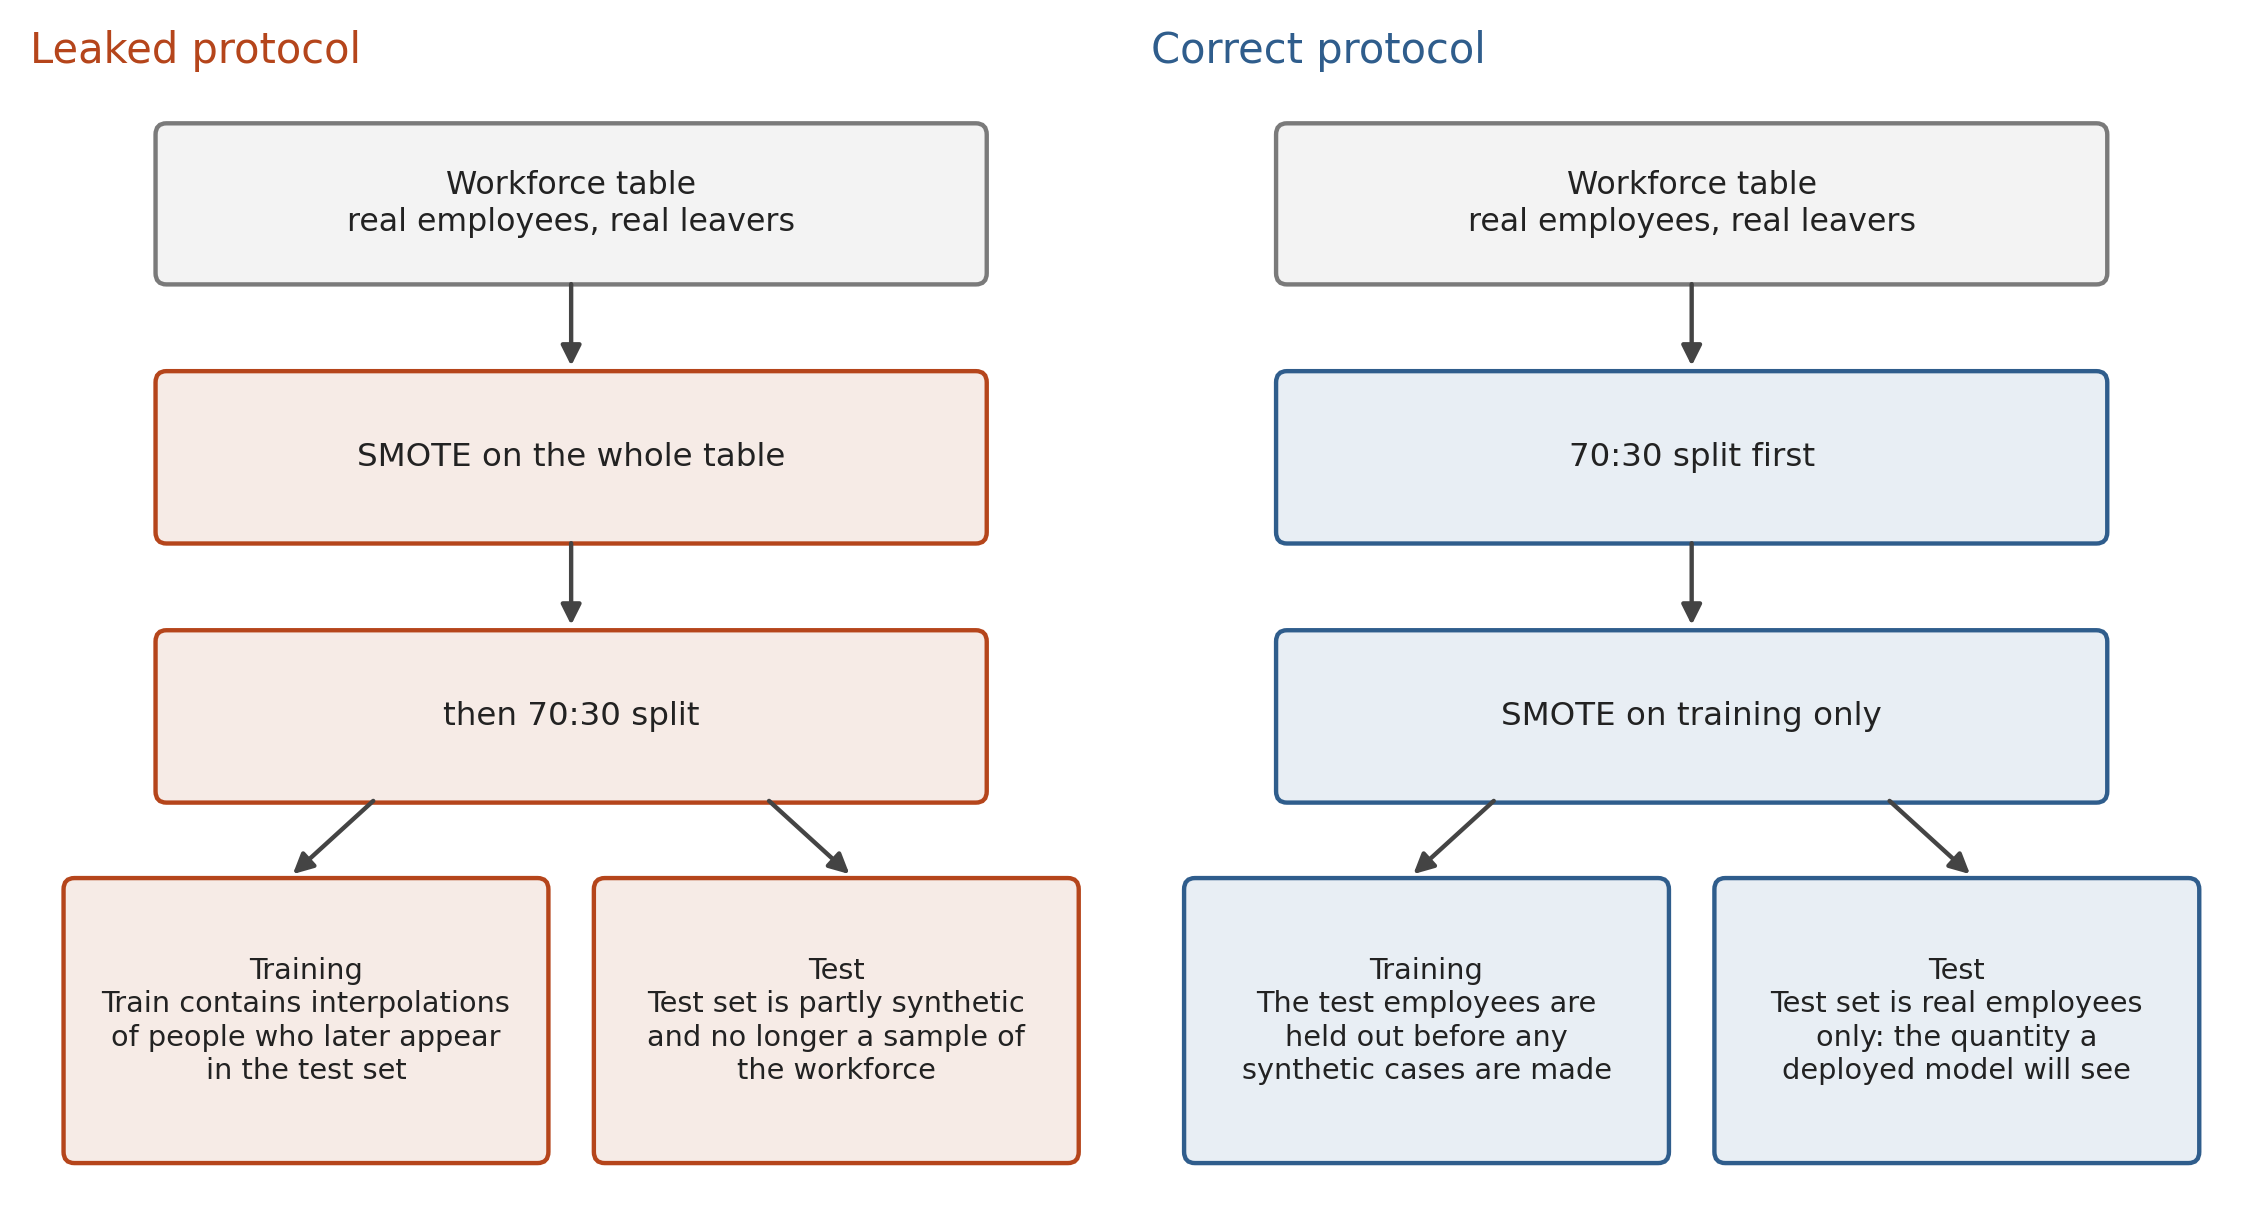
\includegraphics[width=0.96\textwidth,height=0.75\textheight,keepaspectratio]{figures/image1.png}
\end{center}

\clearpage
\refstepcounter{figure}\label{fig:2}
\section*{Figure~\thefigure}
\begin{center}
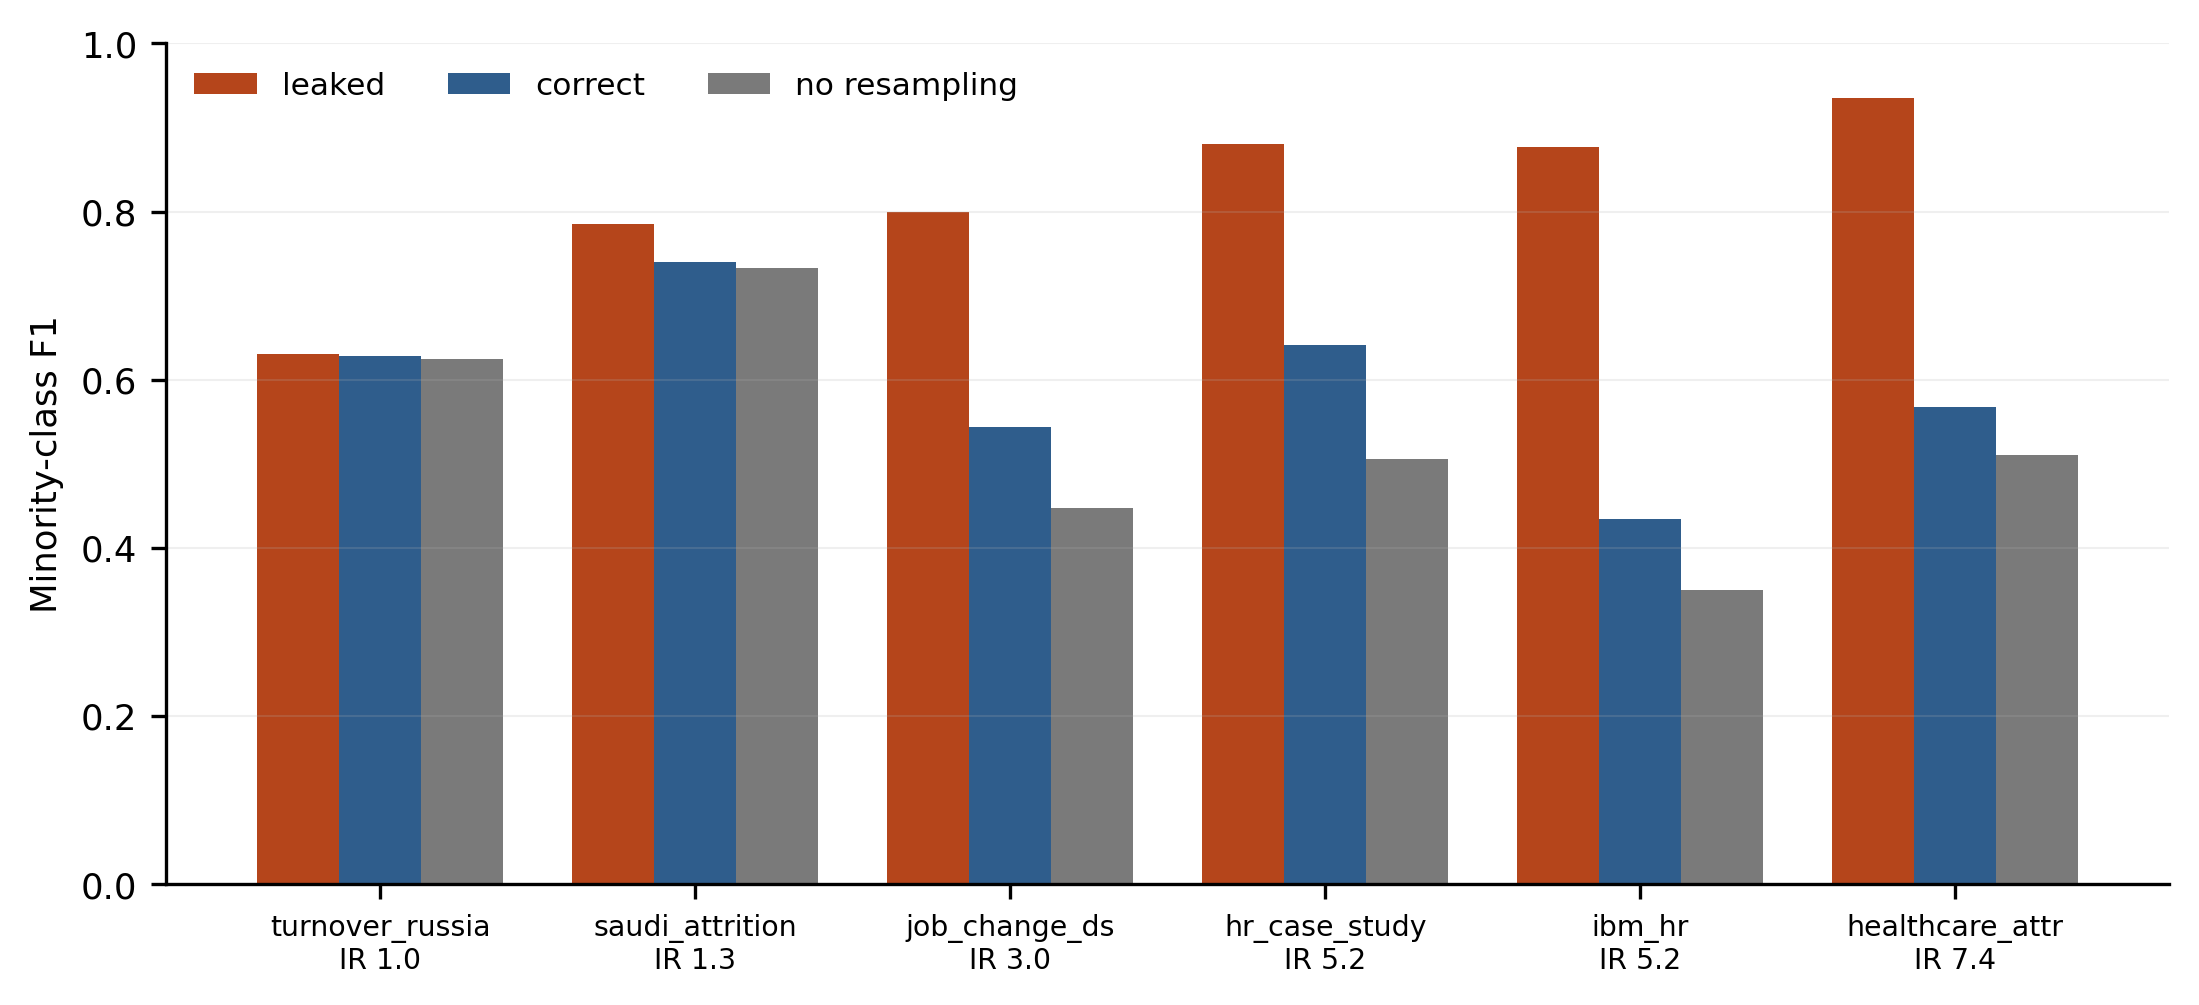
\includegraphics[width=0.96\textwidth,height=0.75\textheight,keepaspectratio]{figures/image2.png}
\end{center}

\clearpage
\refstepcounter{figure}\label{fig:3}
\section*{Figure~\thefigure}
\begin{center}
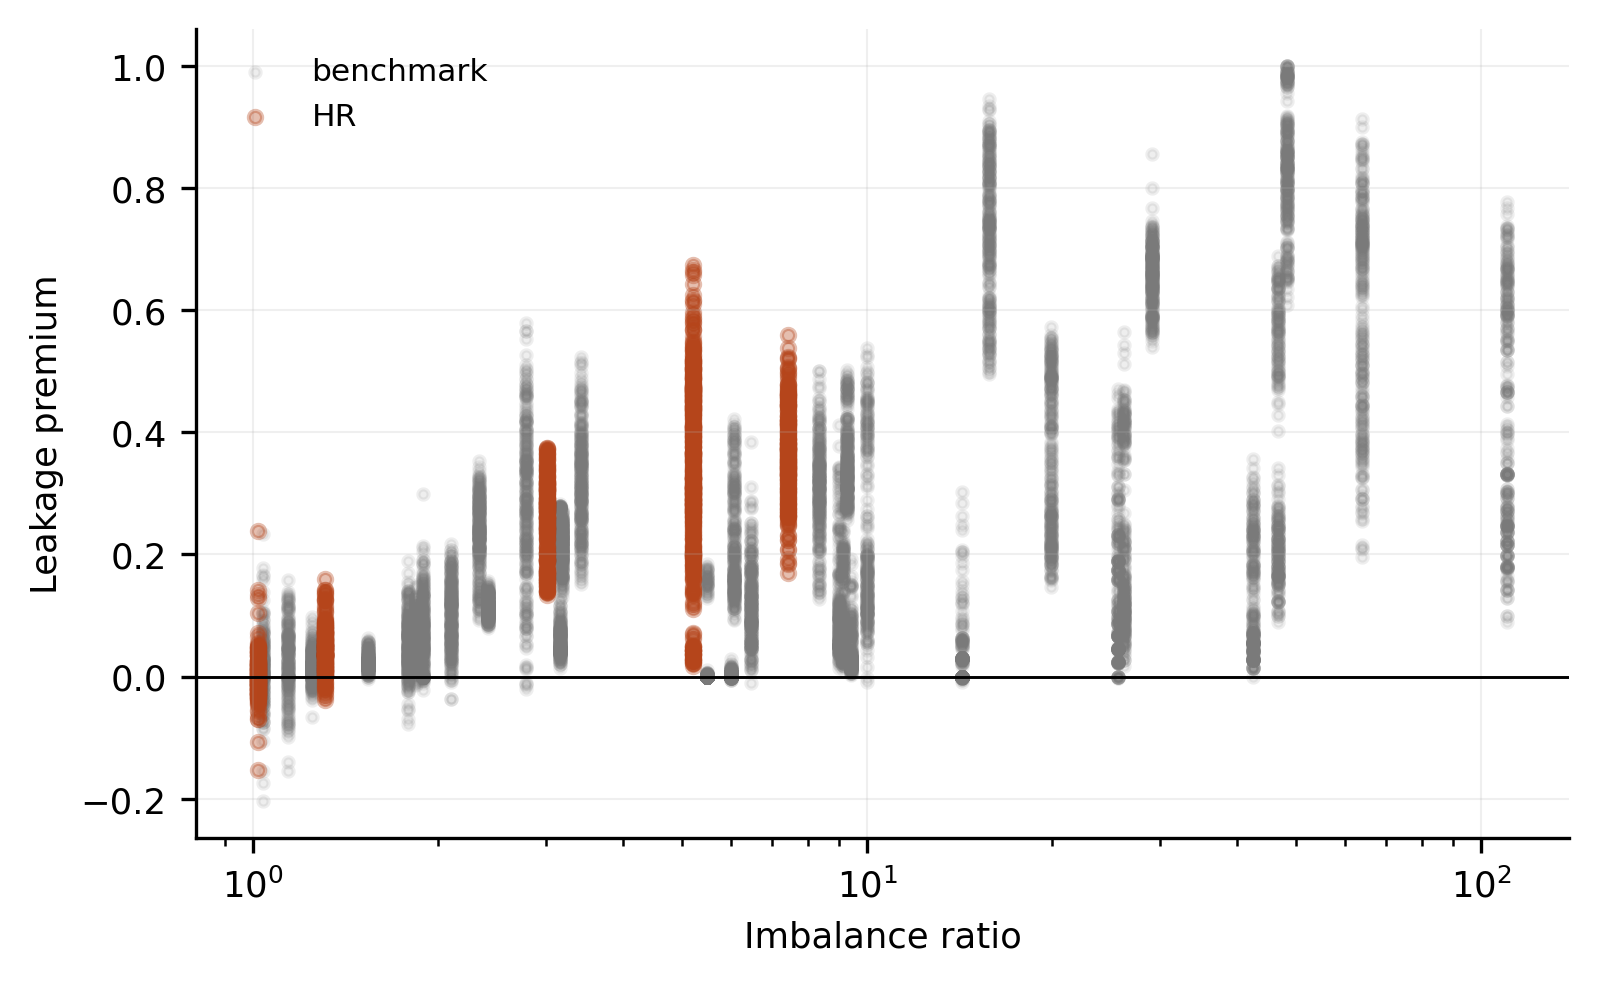
\includegraphics[width=0.96\textwidth,height=0.75\textheight,keepaspectratio]{figures/image3.png}
\end{center}

\clearpage
\refstepcounter{figure}\label{fig:4}
\section*{Figure~\thefigure}
\begin{center}
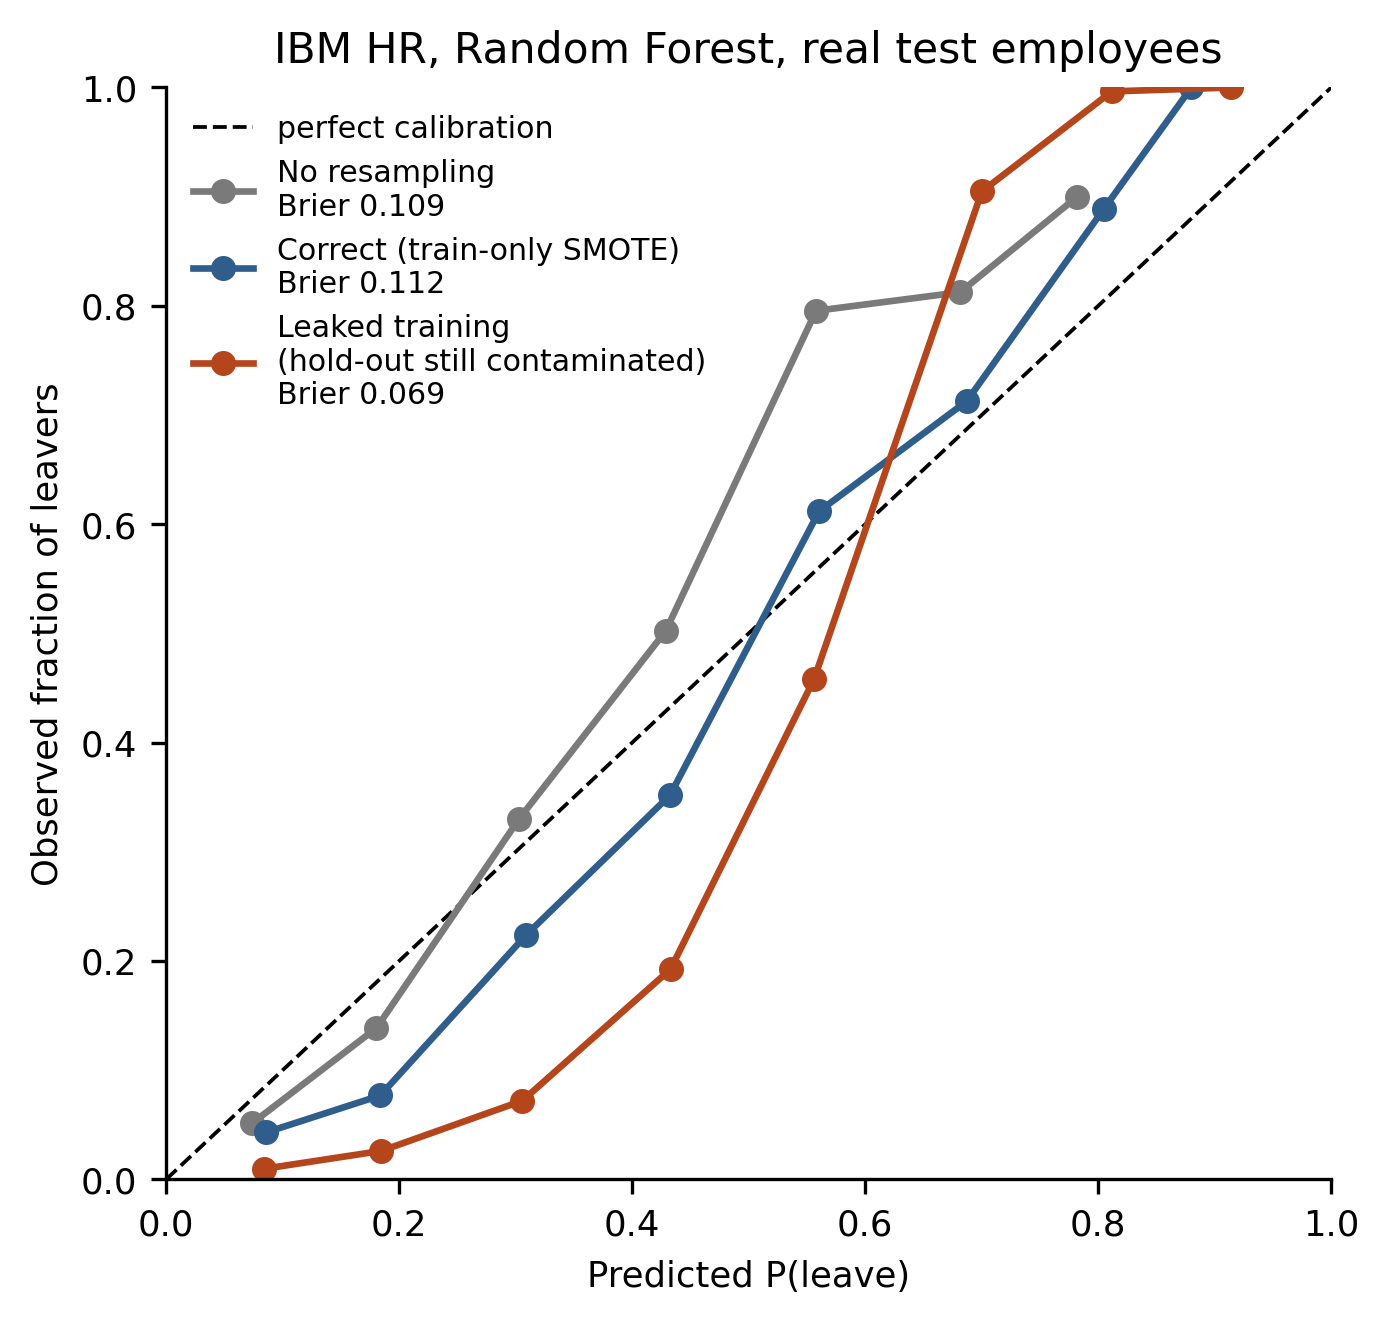
\includegraphics[width=0.96\textwidth,height=0.75\textheight,keepaspectratio]{figures/image4.png}
\end{center}

\clearpage
\section*{Figure captions}
\noindent\textbf{Figure~\ref{fig:1}.} Two evaluation protocols that differ only in where the over-sampler sits. Left: the leaked ordering, in which interpolations of people who later appear in the test set can enter the training partition, and the test set itself is partly synthetic. Right: the correct ordering. Everything else in the experiment---dataset, encoding, classifier, hyperparameters, over-sampler, split proportion, seed---is held fixed.

\noindent\textbf{Figure~\ref{fig:2}.} The three protocols on each employee-turnover dataset, averaged over all classifiers, over-samplers and seeds. Datasets are ordered by imbalance ratio. On the two near-balanced datasets at the left the three protocols agree; as the leaver proportion falls, the leaked bar detaches from the other two and the gap widens to a factor of 2.02 on the IBM benchmark.

\noindent\textbf{Figure~\ref{fig:3}.} The HR datasets against the wider benchmark reference distribution. Each point is one matched comparison and the horizontal axis is the imbalance ratio. Within the HR range the leakage premium climbs steeply with imbalance, demonstrating why the datasets whose turnover prevalence most resembles a real workforce are the ones the protocol error damages most.

\noindent\textbf{Figure~\ref{fig:4}.} Reliability diagram, IBM HR, Random Forest, SMOTE across 10 stratified 70:30 hold-outs ($n_{\text{test}}=441$ real employees per hold-out). Mean $\pm$ SD Brier scores across seeds are $0.1088 \pm 0.0042$ (no resampling), $0.1123 \pm 0.0035$ (correct train-only SMOTE), and $0.0687 \pm 0.0045$ (leaked training). No-resampling and correct series are evaluated on untouched real employees; the leaked series is trained with synthetic interpolations of those same hold-out employees in the training partition, so its apparent calibration is an artefact of contamination rather than future-cohort reliability.

\end{document}
